\documentclass[11pt]{article}
\usepackage[utf8]{inputenc}
\usepackage[pdftex]{graphicx}
\usepackage{pdfpages}
\usepackage{makeidx}
\usepackage[english]{babel}
\usepackage [autostyle, english = american]{csquotes}
\usepackage{mathtools}
\usepackage{xcolor}
\usepackage{listings}
\usepackage{caption,subcaption}
%\usepackage{subfigure}
\usepackage{geometry}
\usepackage{adjustbox}
\usepackage{calc}
\usepackage{ifthen}
\usepackage{listings}
\usepackage{hyperref}
\usepackage[square,sort,comma,numbers]{natbib}
\usepackage{cleveref}
\usepackage[section,cachedir=build,newfloat]{minted}
\usepackage{chngcntr}
\usepackage[cm]{fullpage}

\definecolor{mintedbackground}{rgb}{0,0,0}


\usemintedstyle{tango}
\newenvironment{code}{\captionsetup{type=listing}}{}
\SetupFloatingEnvironment{listing}{name=Source Code}
\captionsetup[subfigure]{subrefformat=simple,labelformat=simple}

\renewcommand{\thelisting}{\arabic{listing}}
\renewcommand\thesubfigure{(\alph{subfigure})}

\bibliographystyle{abbrvnat}

\geometry{
 a4paper,
 total={170mm,257mm},
 left=20mm,
 top=20mm,
}

\definecolor{lightgray}{rgb}{.7,.7,.7}
\definecolor{gray}{rgb}{.4,.4,.4}
\definecolor{darkblue}{rgb}{0,0,.3}
\definecolor{gray}{rgb}{0.4,0.4,0.4}
\definecolor{darkblue}{rgb}{0.0,0.0,0.6}
\definecolor{cyan}{rgb}{0.0,0.6,0.6}

\lstset{
  basicstyle=\ttfamily,
  columns=fullflexible,
  showstringspaces=false,
  commentstyle=\color{gray}\upshape
}

\lstdefinelanguage{XML}
{
  morestring=[b]",
  morestring=[s]{>}{<},
  morecomment=[s]{<?}{?>},
  stringstyle=\color{black},
  identifierstyle=\color{darkblue},
  keywordstyle=\color{cyan},
  morekeywords={xmlns,version,type}% list your attributes here
}
 
 
\hypersetup{
    colorlinks,
    citecolor=black,
    filecolor=black,
    linkcolor=black,
     urlcolor=blue
}
 


\newmintedfile[pycode]{python3}{
frame=lines,
framesep=2mm,
fontsize=\footnotesize,
showtabs =false,
autogobble=true,
breaklines=true,
mathescape=true
}

\newmintedfile[rcode]{S}{
frame=lines,
framesep=2mm,
fontsize=\footnotesize,
showtabs =false,
autogobble=true,
breaklines=true,
mathescape=true
}

\title{Assignment 2 \\ Introduction to Information Retrieval \\ CS734/834}
\author{John Berlin}
\date{\today}
\renewcommand\thesection{Q.\arabic{section}}
\renewcommand\thesubsection{\thesection}
\begin{document}
\maketitle
\newpage
\section*{Note}
In order to make processing of the Wiki dataset timely and repeatable the util python file \autoref{code:util}, was utilized to serialize the files full paths to disk in \href{https://docs.python.org/3/library/pickle.html}{pickle} format. Also included in this serialization was a python set of Wiki articles for both small and large datasets, this was necessary to ensure that self links were included when doing the calculations for \autoref{q:pr}. The pickle format was used for the questions involving the Wiki dataset size allowing. Graphv3 generated by \autoref{q:pr} is not included with this report as Github does not like large files, its size is 436mb compressed likewise the inverted index for wiki-large is not included as its size if 1.6gb uncompressed in pickle format. 

\section{Question 4.2}
\begin{verbatim}
Plot vocabulary growth for the Wikipedia collection and estimate the pa-
rameters for Heaps’ law. Should the order in which the documents are processed
make any difference?
\end{verbatim}
\subsection{Answer}
\begin{figure}[h]
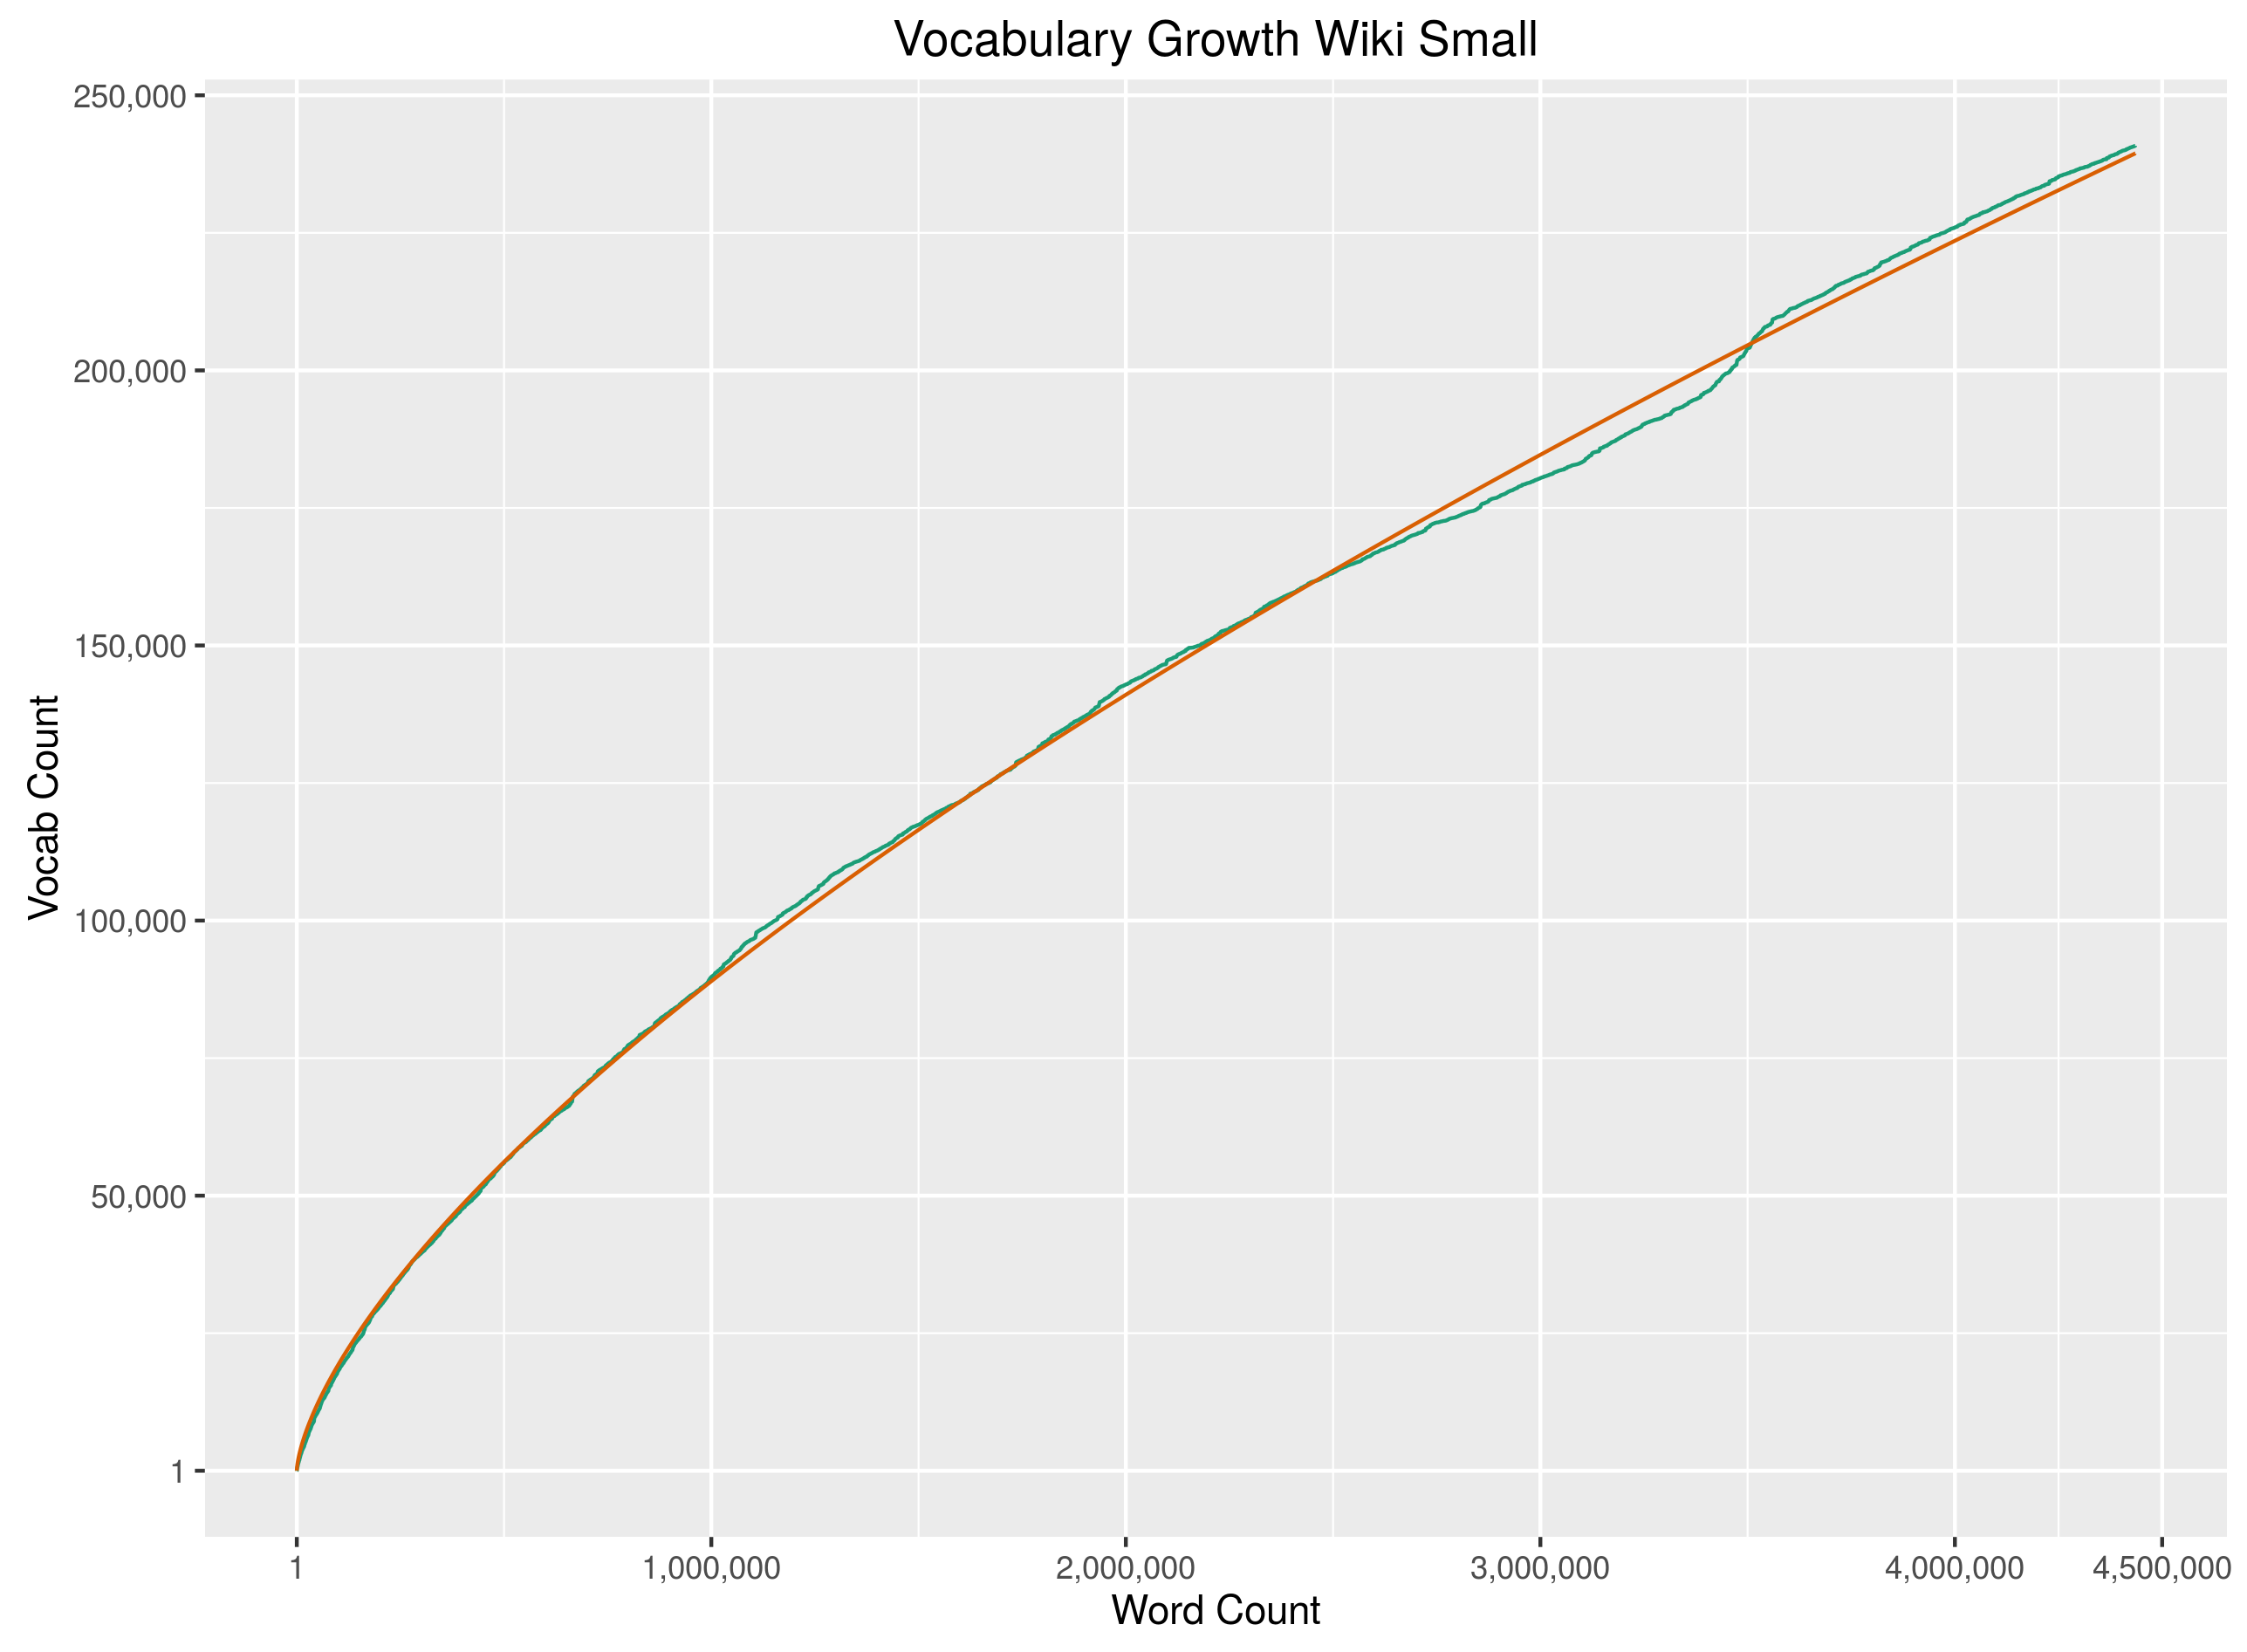
\includegraphics[width=\columnwidth]{code/wikiSmallVG.png}
\caption{Wiki Small Vocab Growth}
\label{fig:wsvg}
\end{figure}
\begin{figure}[h]
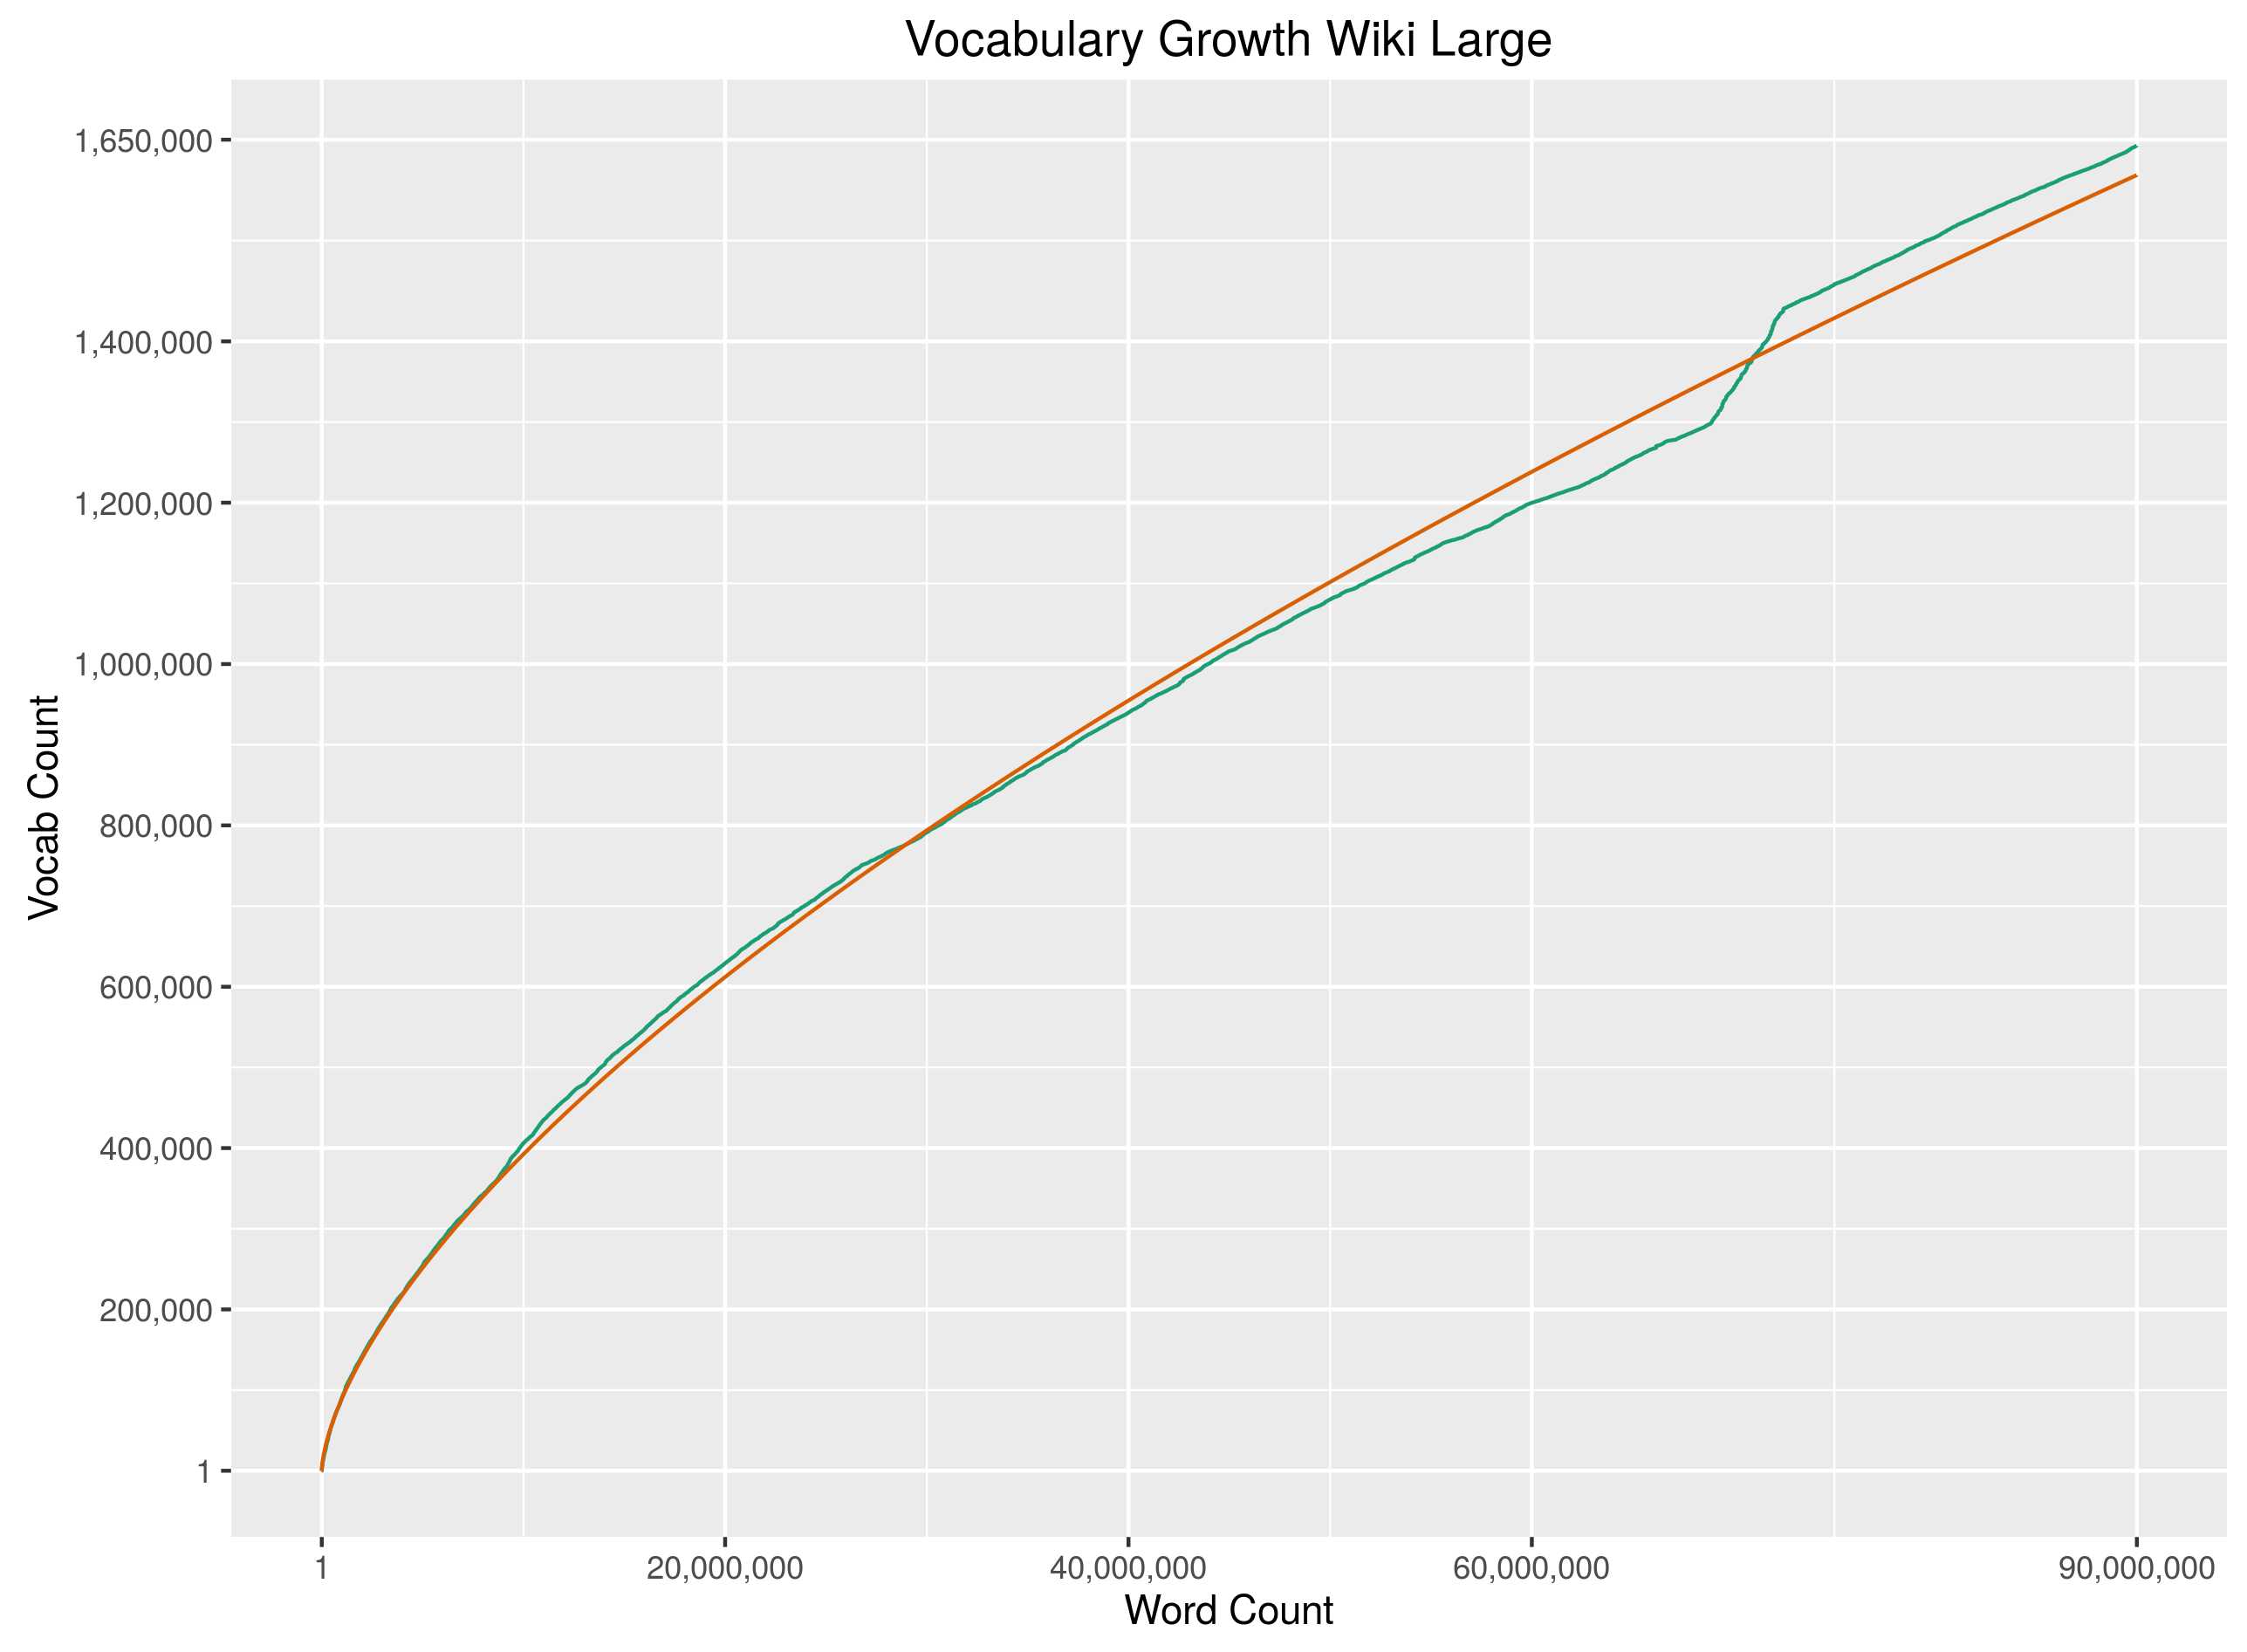
\includegraphics[width=\columnwidth]{code/wikiLargeVG.png}
\caption{Wiki Large Vocab Growth}
\label{fig:wsvg}
\end{figure}
\begin{figure}[h]
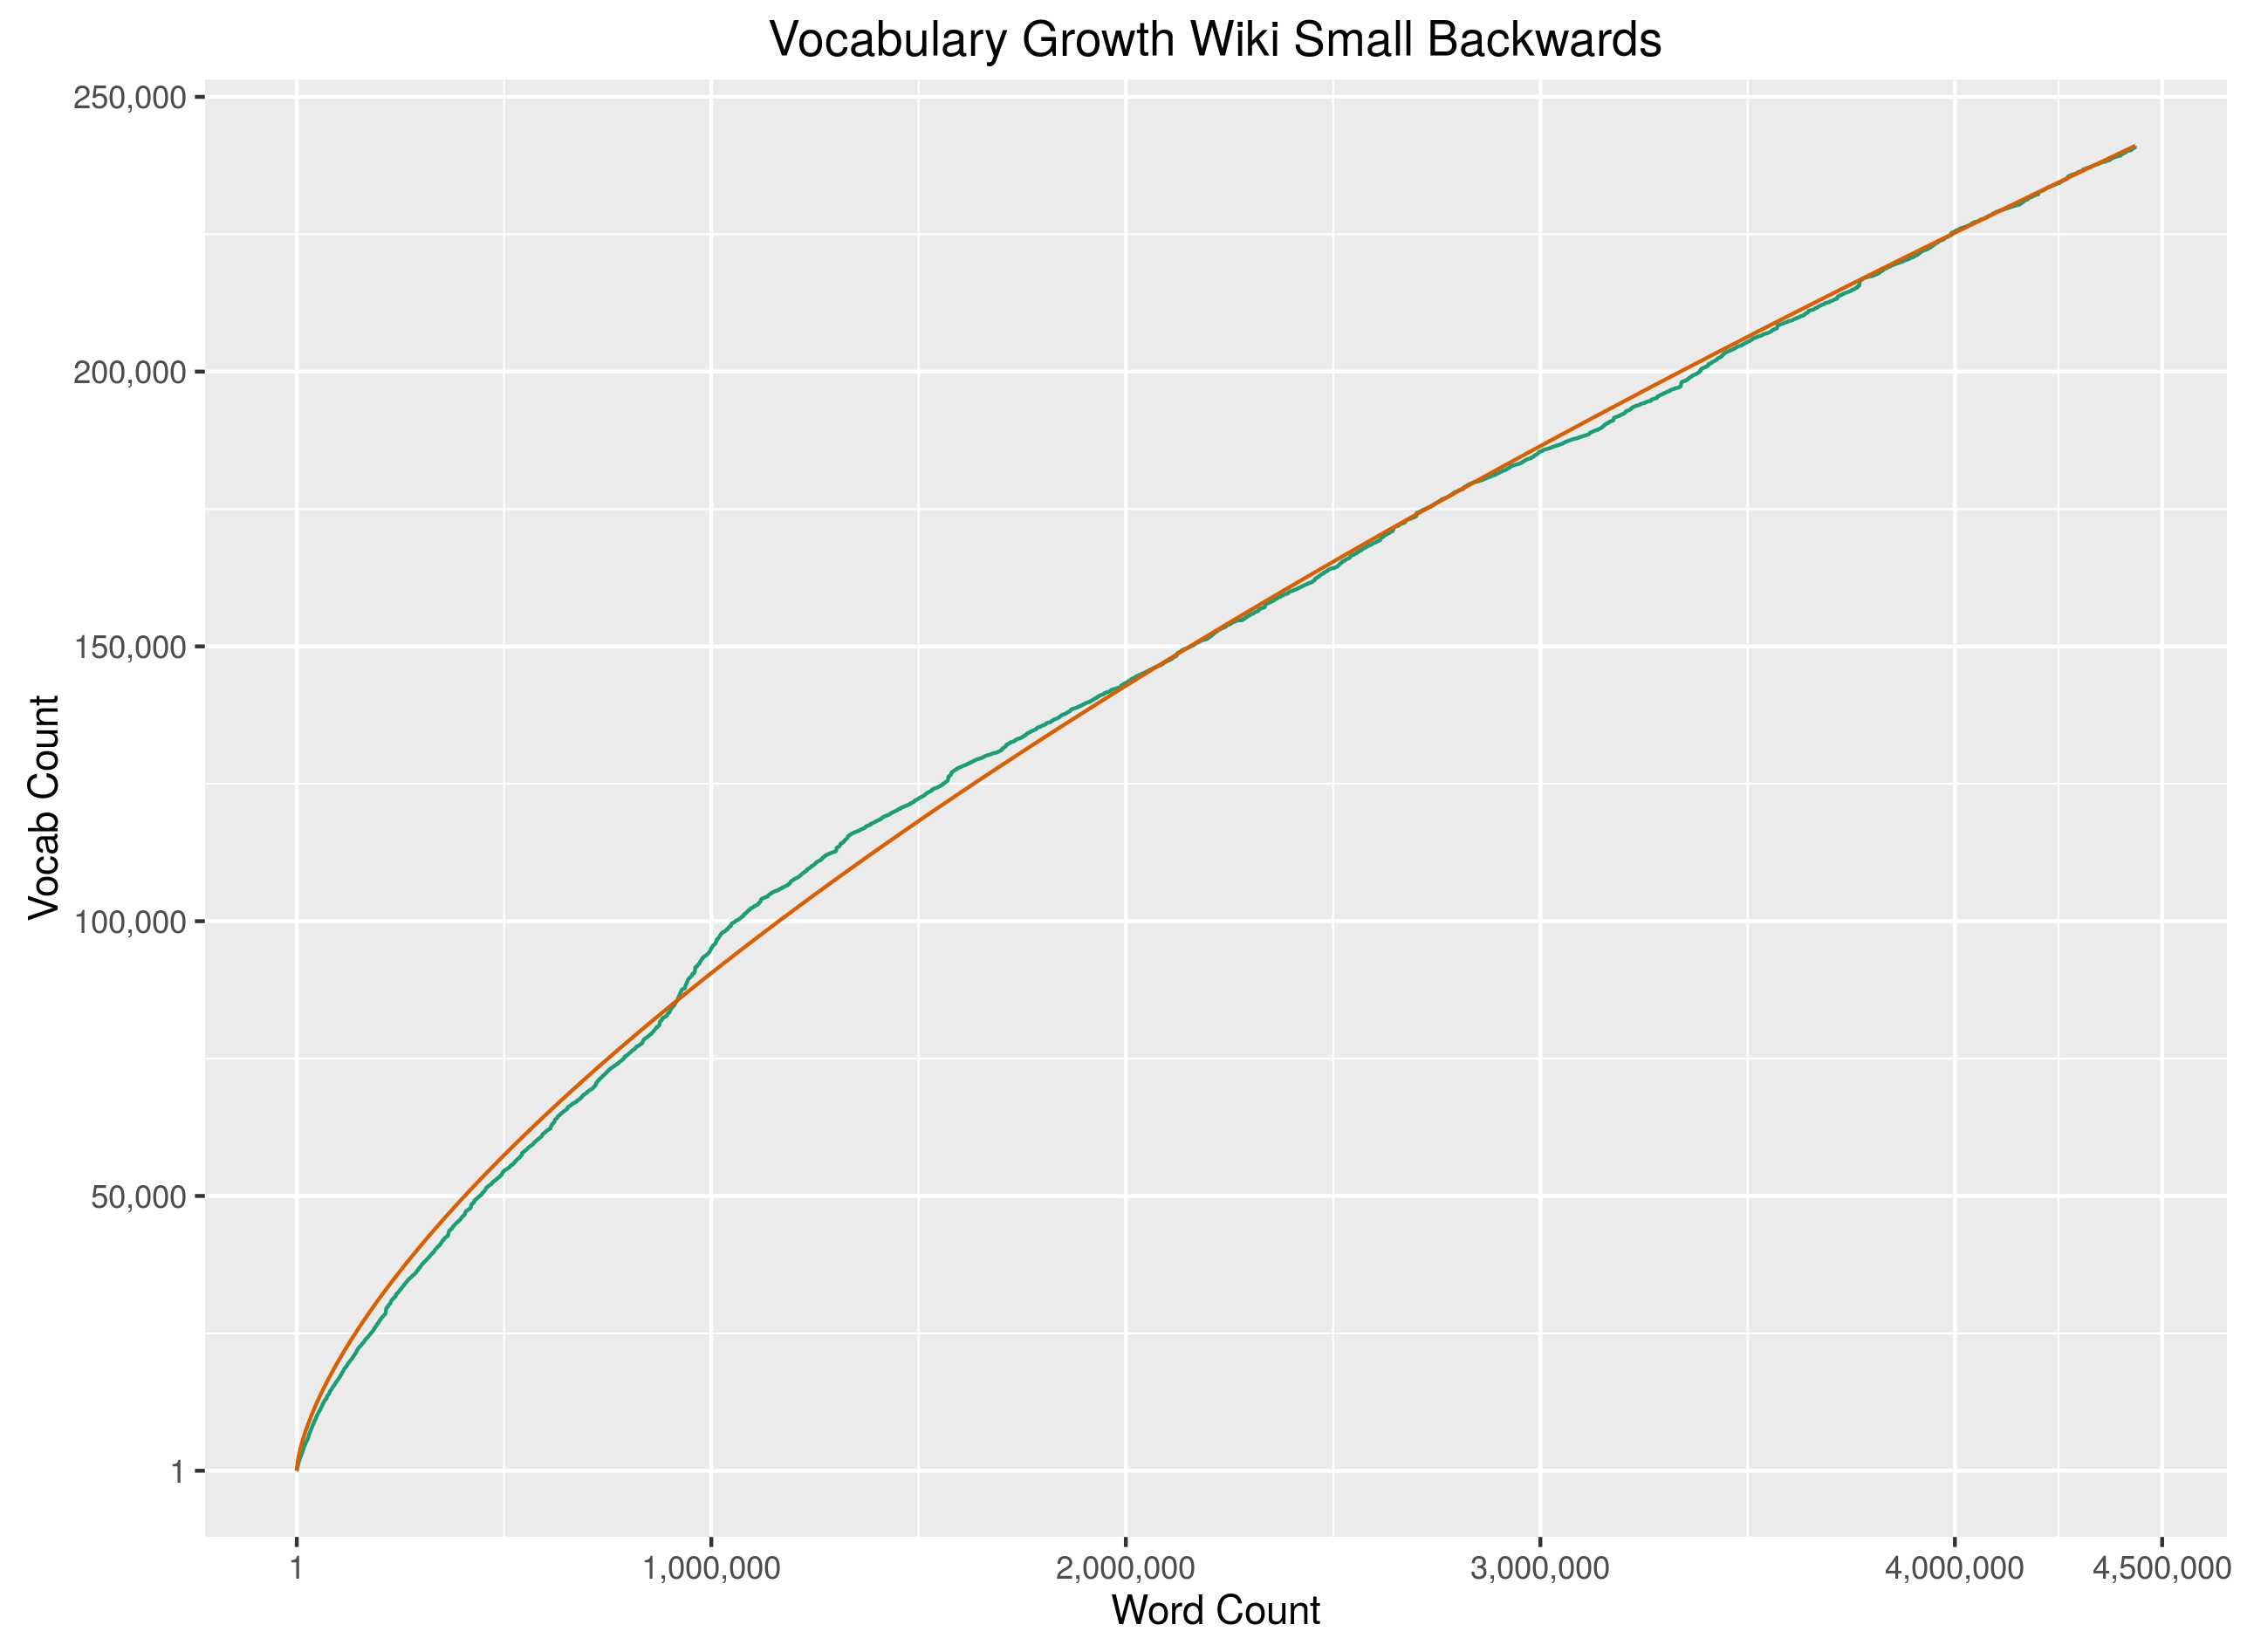
\includegraphics[width=\columnwidth]{code/wikiSmallVGB.png}
\caption{Wiki Small Vocab Growth Reverse Order}
\label{fig:wsvgb}
\end{figure}
\begin{figure}[h]
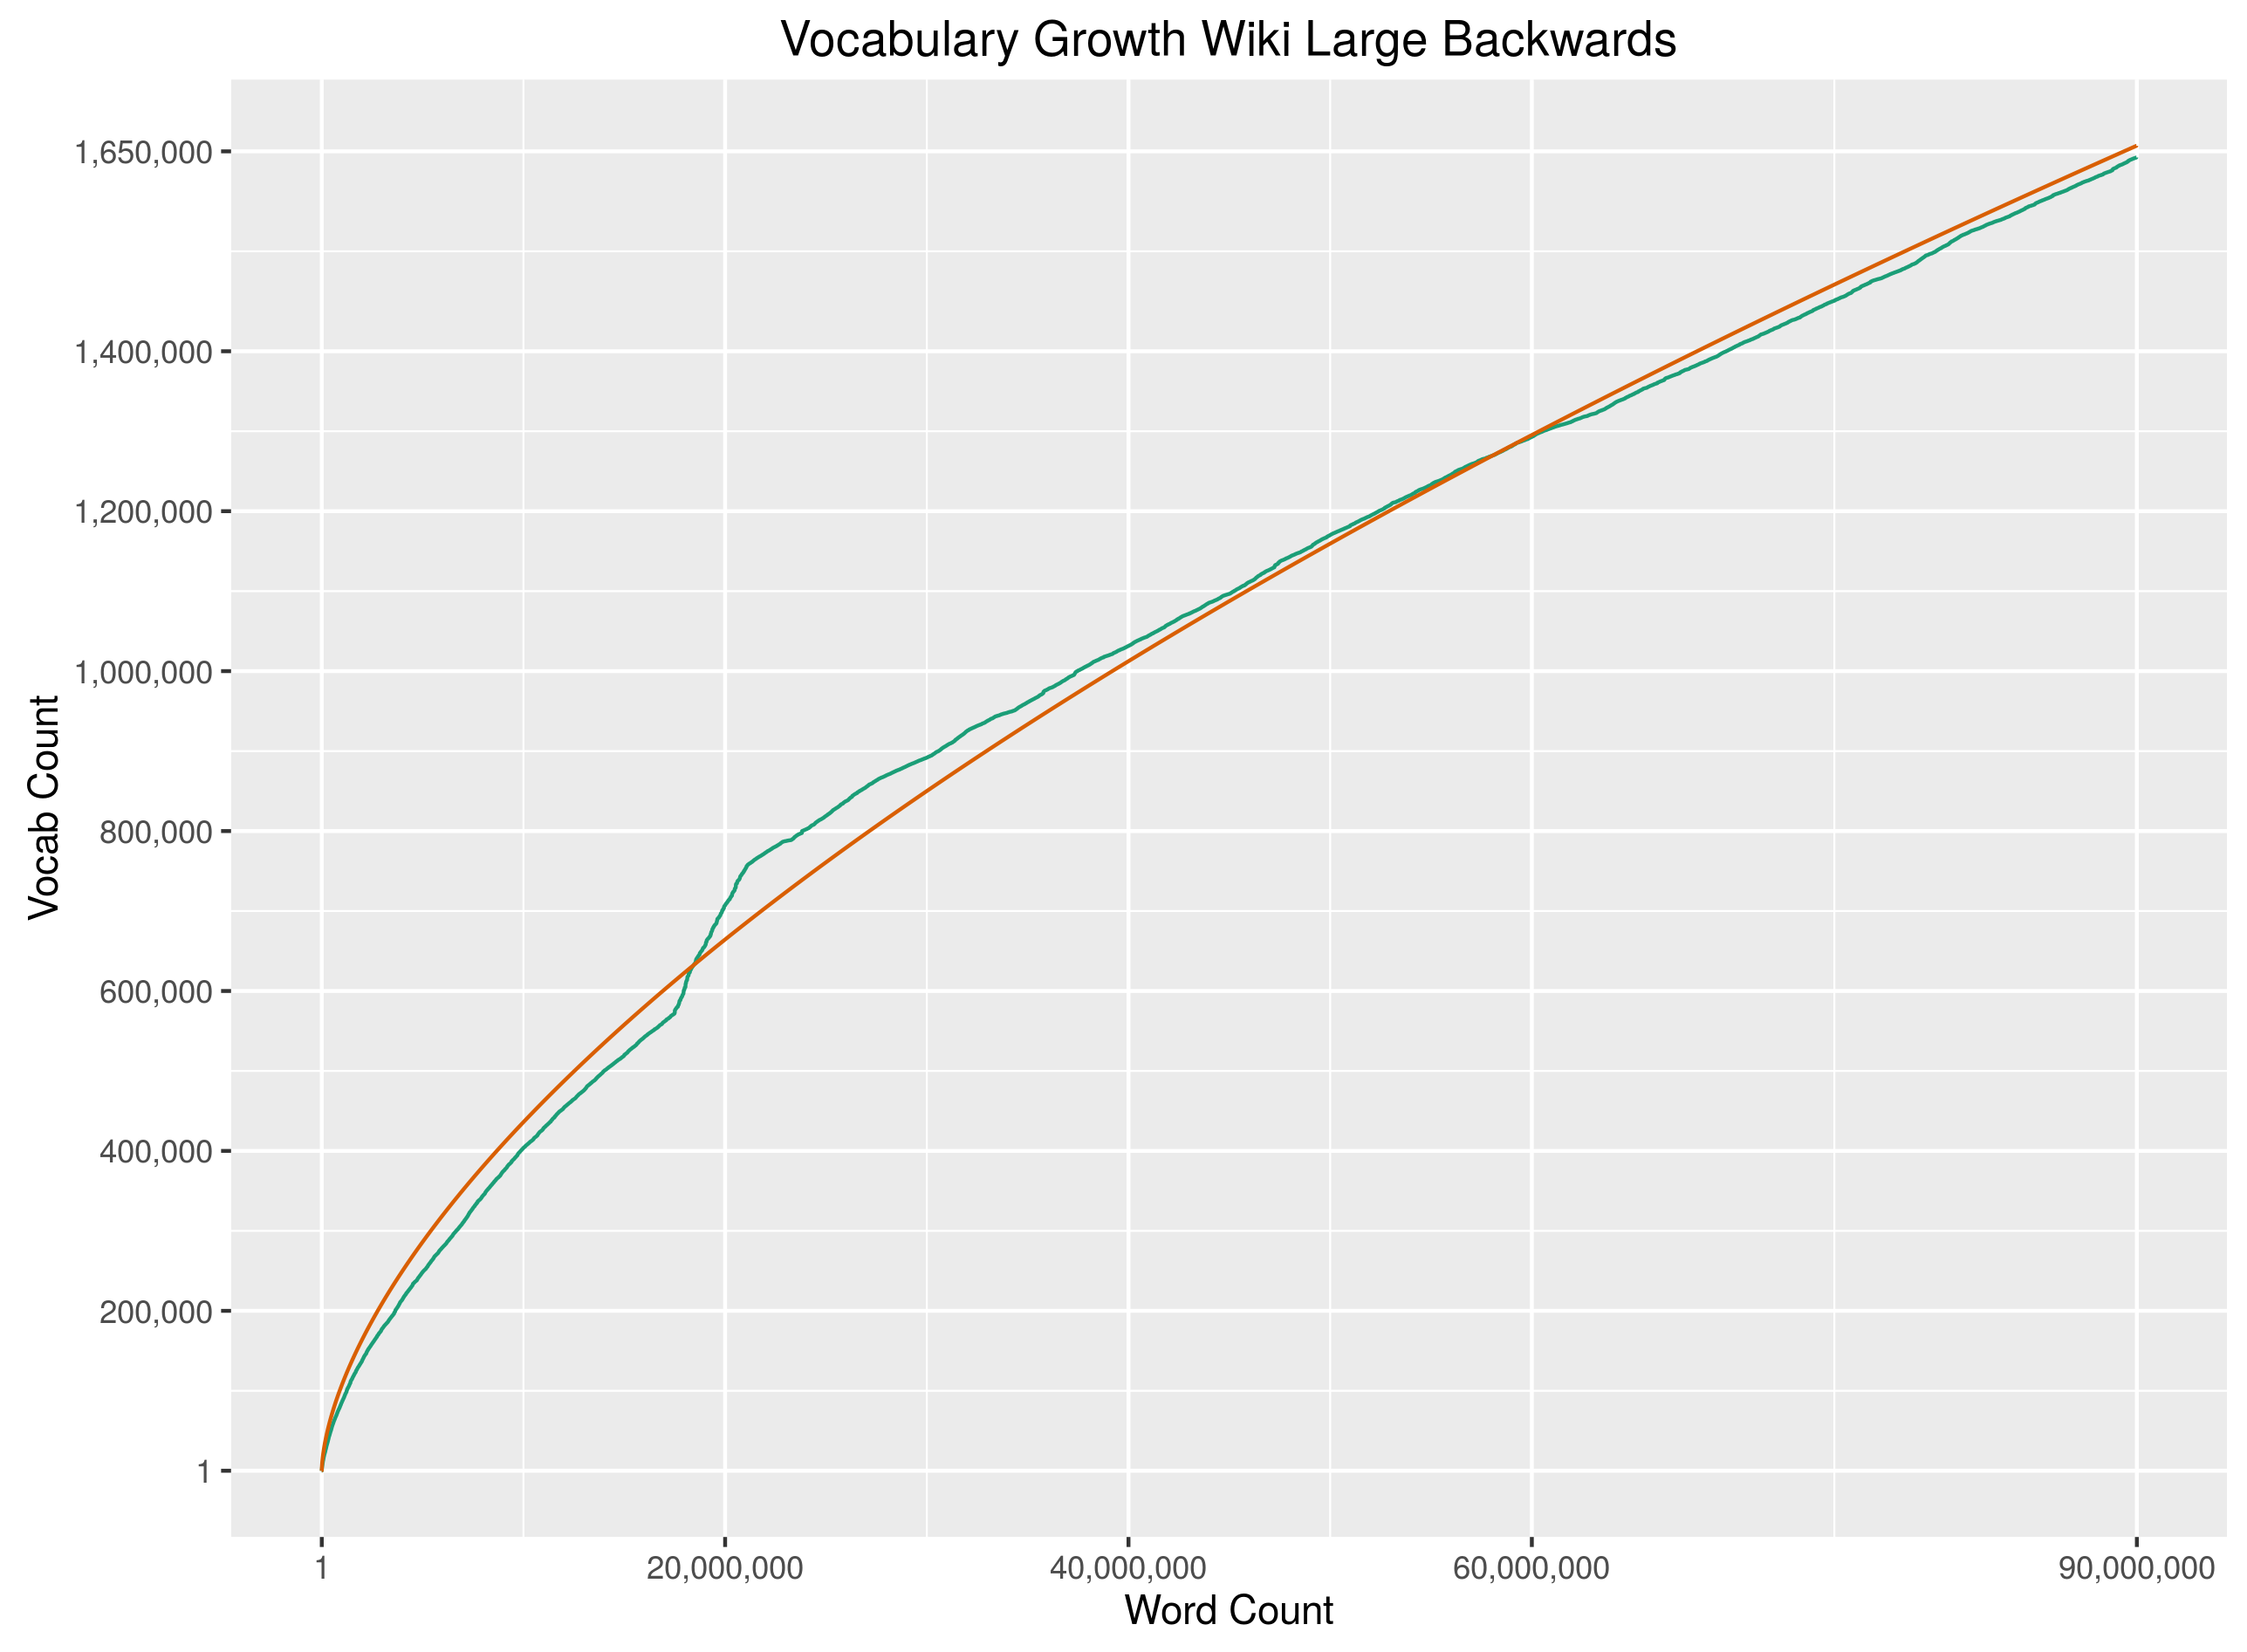
\includegraphics[width=\columnwidth]{code/wikiLargeVGB.png}
\caption{Wiki Large Vocab Growth Reverse Order}
\label{fig:wlvgb}
\end{figure}
\begin{figure}[h]
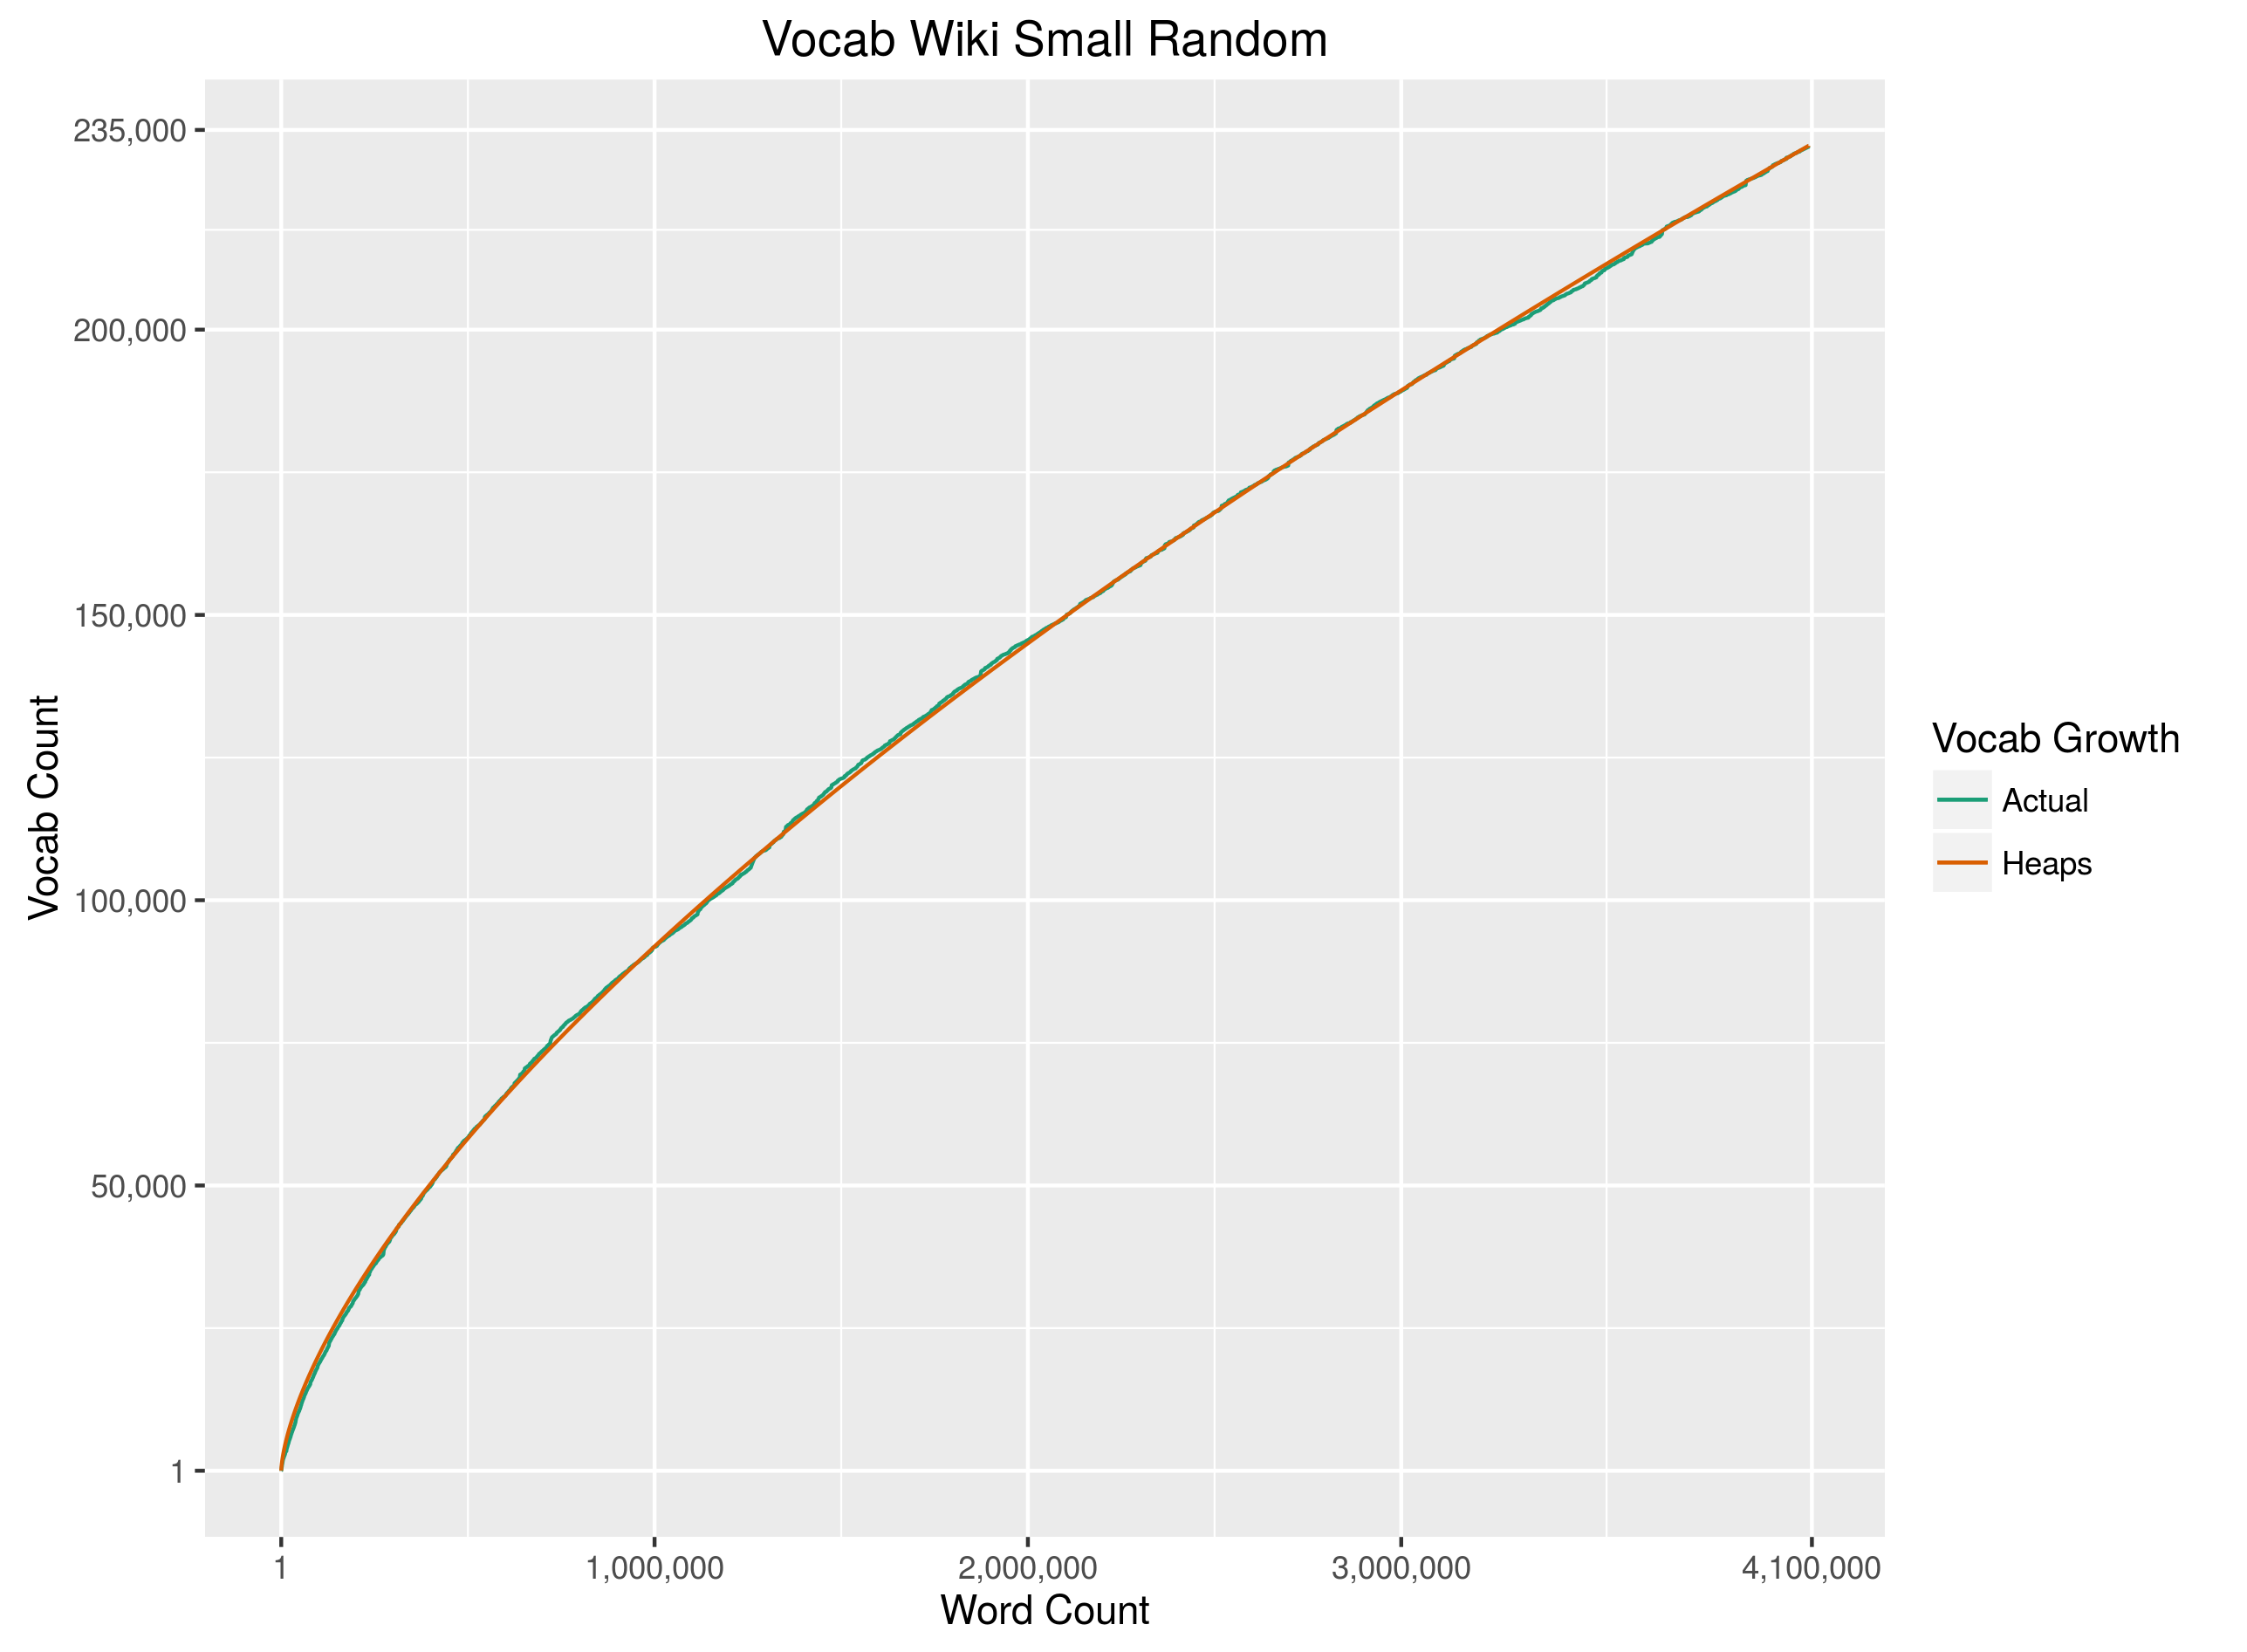
\includegraphics[width=\columnwidth]{code/wikiSmallVR.png}
\caption{Wiki Small Vocab Growth Random Order}
\label{fig:wsvgr}
\end{figure}
\begin{figure}[h]
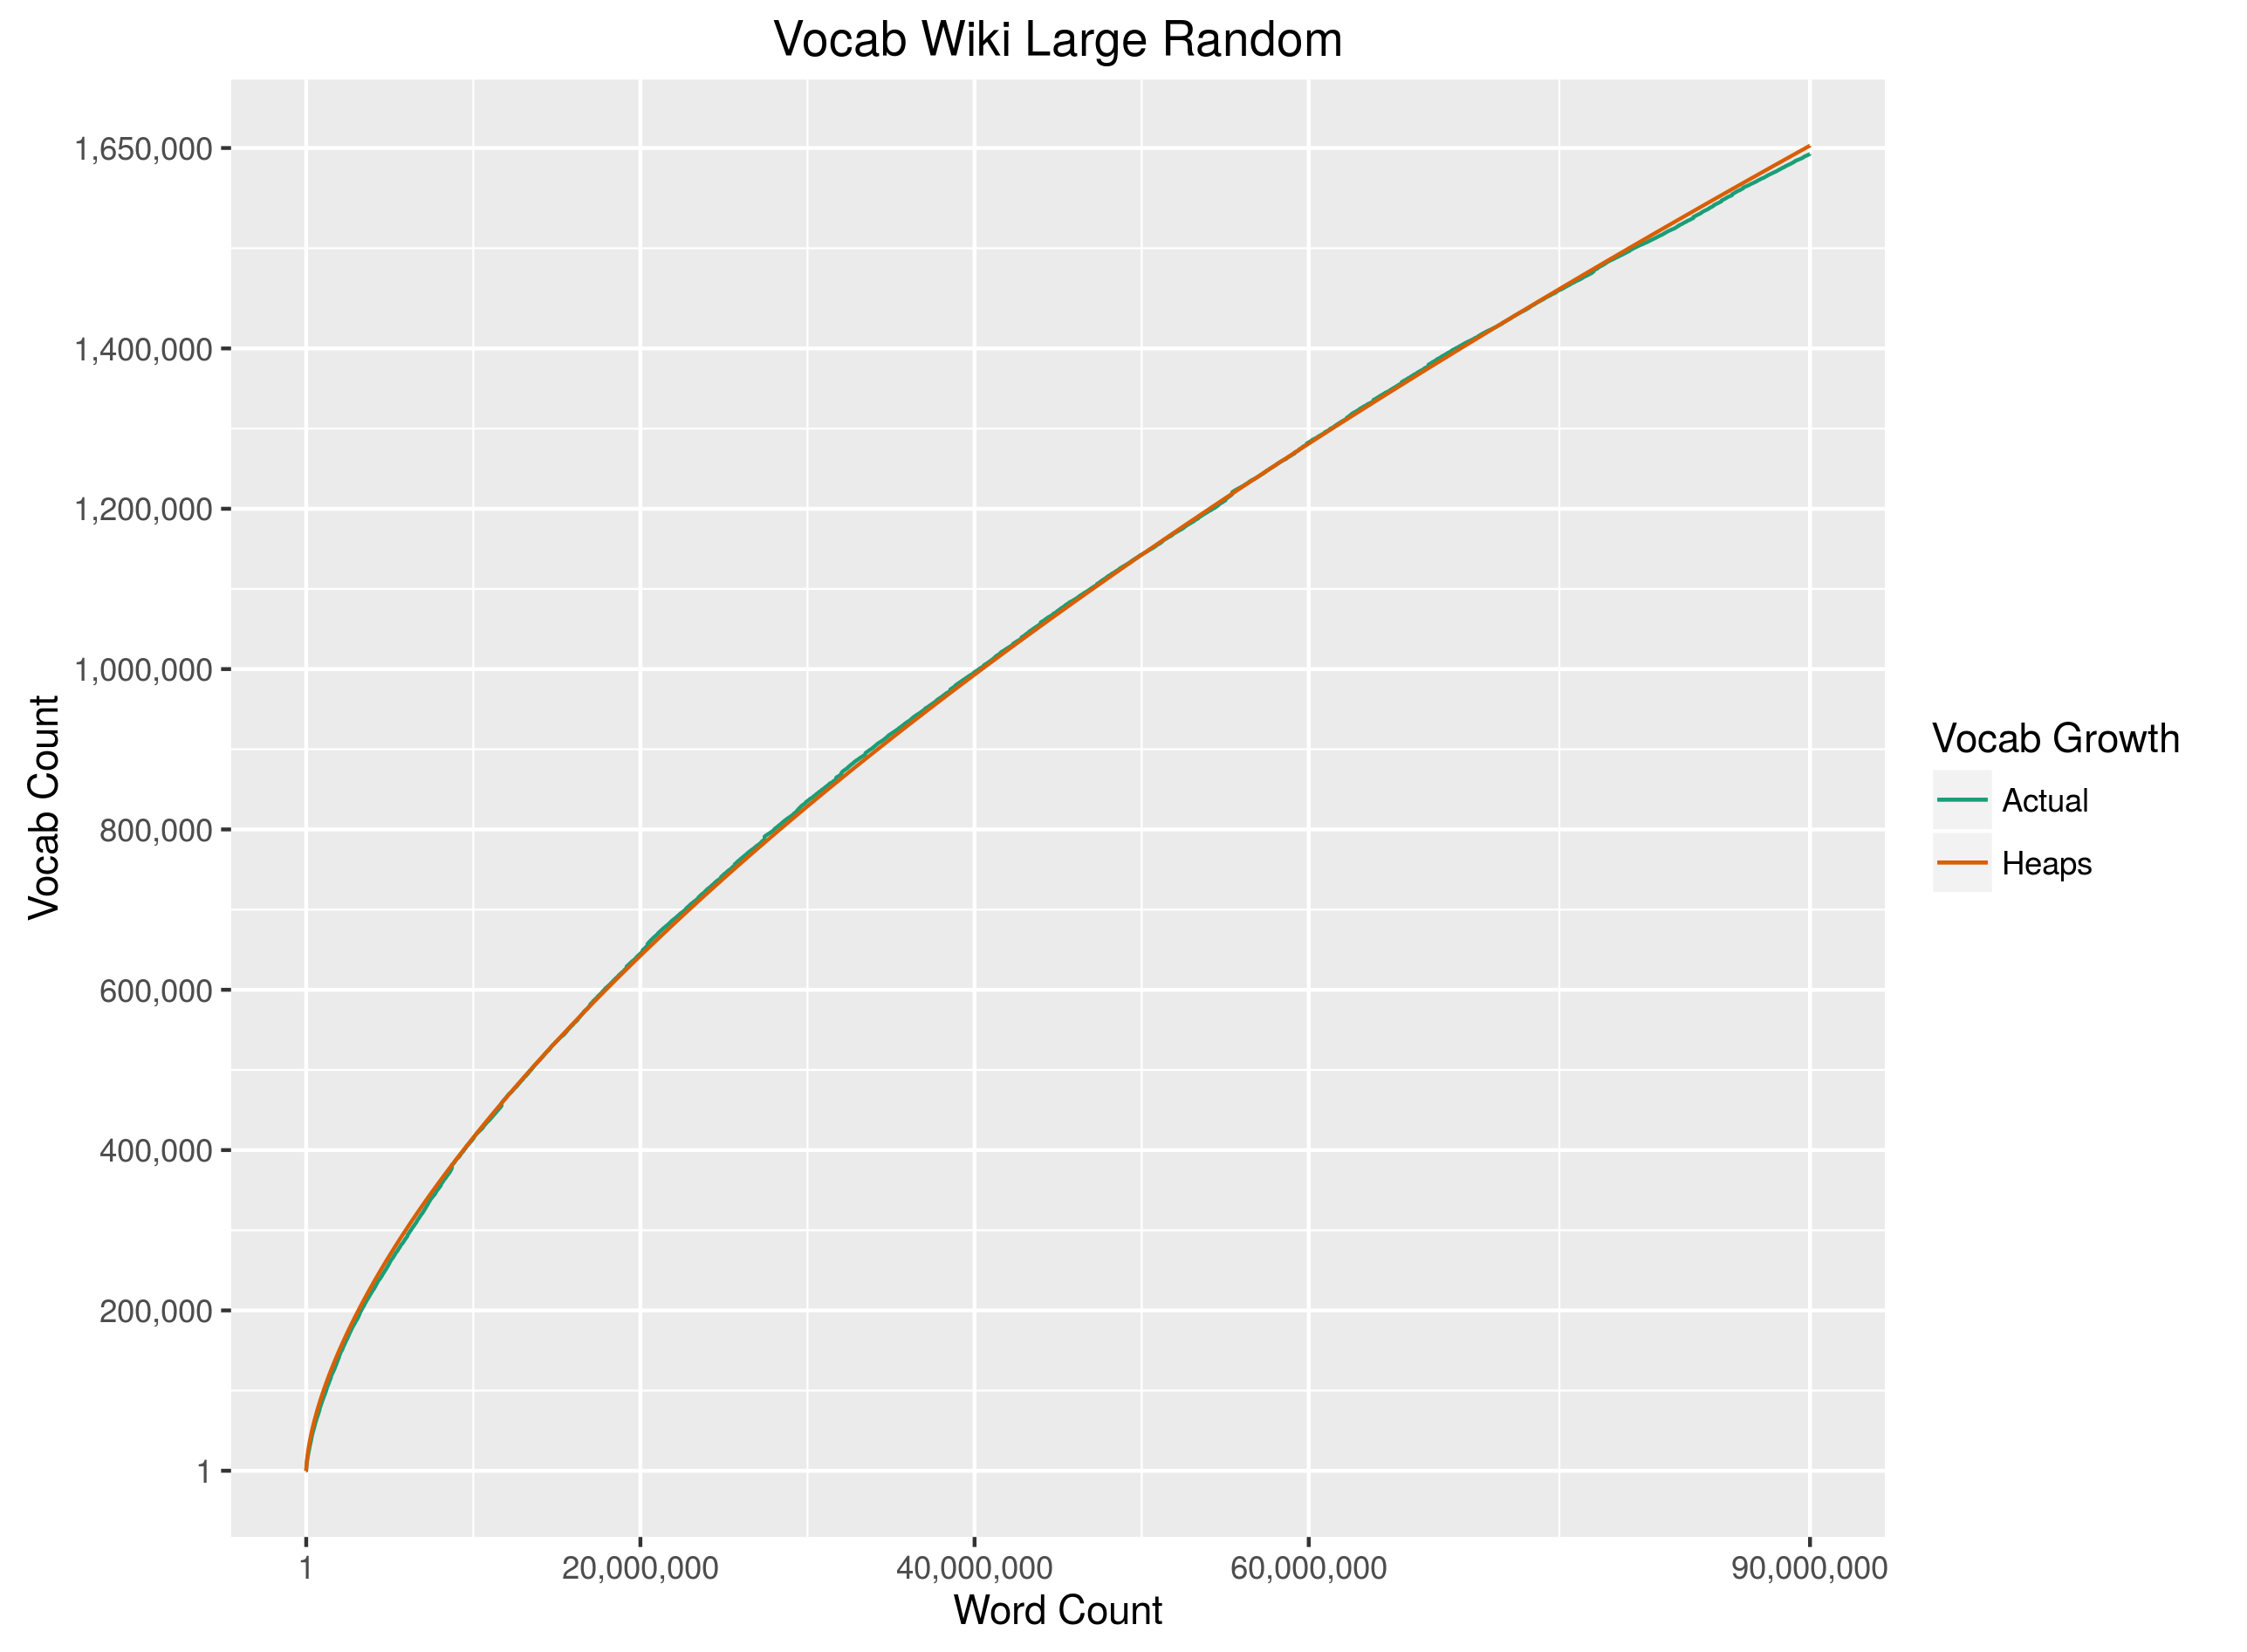
\includegraphics[width=\columnwidth]{code/wikiLargeVGR.png}
\caption{Wiki Large Vocab Growth Random Order}
\label{fig:wlvgr}
\end{figure}
\newpage
\clearpage
\begin{code}
	\pycode{code/wiki_vocab.py}
	\captionof{listing}{Wiki Vocab Processing Code} \label{code:vcp}
\end{code}

\newpage
\begin{code}
	\rcode{code/wiki-vocab.R}
	\captionof{listing}{Wiki Vocab Plot Code} \label{code:vcr}
\end{code}
\newpage
\section{Question 4.9}
\label{q:pr}
\begin{verbatim}
Compute PageRank for the Wikipedia documents. List the 20 documents
with the highest PageRank values together with the values.
\end{verbatim}
\subsection{Answer}
\begin{code}
	\pycode{code/wiki_pagerank.py}
	\captionof{listing}{Wiki PageRank Code} \label{code:pr}
\end{code}
\begin{table}[h]
\centering
\caption{Wiki Top 20 Page Rank}
\label{tb:wpr} 
\begin{minipage}{.5\textwidth}
\begin{tabular}{lc|}
\multicolumn{1}{c}{Wiki Small Page} & \multicolumn{1}{c|}{rank} \\
Brazil.html & 0.01739 \\
Fernando\_Collor\_de\_Mello\_1c42.html & 0.01497 \\
August\_26.html & 0.00963 \\
Kidney.html & 0.00620 \\
Diabetic\_nephropathy.html & 0.00537 \\
Seinfeld.html & 0.00201 \\
Ronald\_Colman\_8c1a.html & 0.00184 \\
Manga.html & 0.00172 \\
Magazine.html & 0.00166 \\
Broderick\_Crawford\_c49a.html & 0.00166 \\
1150.html & 0.00154 \\
Pope\_Innocent\_VIII\_650a.html & 0.00149 \\
Transjordan.html & 0.00147 \\
Gilbert\_and\_Ellice\_Islands\_8a4e.html & 0.00147 \\
Mollusca.html & 0.00145 \\
Pope\_Paul\_VI\_4529.html & 0.00143 \\
List\_of\_Navarrese\_monarchs\_334f.html & 0.00140 \\
F-102\_Delta\_Dagger\_058e.html & 0.00136 \\
Isthmian\_League\_1d48.html & 0.00136 \\
Pope\_Benedict\_IV\_b5de.html & 0.00135
\end{tabular}
 \end{minipage}%
    \begin{minipage}{0.5\textwidth}
    \begin{tabular}{lc}
\multicolumn{1}{c}{Wiki Large Page} & rank \\
Record\_label.html & 0.00855 \\
Music\_genre.html & 0.00812 \\
London.html & 0.00767 \\
UTC-5\_c184.html & 0.00551 \\
Brazil.html & 0.00498 \\
Radio.html & 0.00469 \\
UTC+2\_8d21.html & 0.00460 \\
Paris.html & 0.00460 \\
1966.html & 0.00383 \\
Romania.html & 0.00329 \\
The\_Byrds\_72ba.html & 0.00306 \\
1962.html & 0.00304 \\
1946.html & 0.00300 \\
July\_1.html & 0.00291 \\
UTC+7$\sim$30\_a9b0.html & 0.00282 \\
Herb\_Alpert\_5b74.html & 0.00281 \\
UTC+5\_6f4a.html & 0.00258 \\
UTC-10\_755d.html & 0.00255 \\
April\_15.html & 0.00251 \\
1930.html & 0.00240
\end{tabular}
\end{minipage}
\end{table}
\newpage
\begin{code}
	\pycode{code/wiki_pagerank.py}
	\captionof{listing}{Wiki PageRank Code} \label{code:pr}
\end{code}

\newpage
\section{Question 4.8}
\begin{verbatim}
Find the 10 Wikipedia documents with the most inlinks. Show the collec-
tion of anchor text for those pages
\end{verbatim}
\subsection{Answer}
\begin{code}
	\pycode{code/wiki-inlinks.py}
	\captionof{listing}{Wiki Inlink Code} \label{code:wil}
\end{code}
\newpage

\section{Question 5.8}
\begin{verbatim}
Write a program that can build a simple inverted index of a set of text docu-
ments. Each inverted list will contain the file names of the documents that contain
that word. (Dr. MLN: use examples from the Wikipedia data set) 
\end{verbatim}
\subsection{Answer}
\begin{code}
	\pycode{code/wikis_inverted_idx.py}
	\captionof{listing}{Wiki Inverted Index Code} \label{code:iidx}
\end{code}
\newpage
\section{Question 5.14}
\begin{verbatim}
In section 5.7.3, we saw that the optimal skip distance c can be determined
by minimizing the quantity kn/c + pc/2, where k is the skip pointer length, n
is the total inverted list size, c is the skip interval, and p is the number of postings
to find.
Plot this function using k = 4, n = 1,000,000, and p = 1,000, but varying c.
Then, plot the same function, but set p = 10,000. Notice how the optimal value
for c changes.
Finally, take the derivative of the function kn/c + pc/2 in terms of c to find
the optimum value for c for a given set of other parameters (k, n, and p).
\end{verbatim}
\subsection{Answer}
\begin{figure}[h]
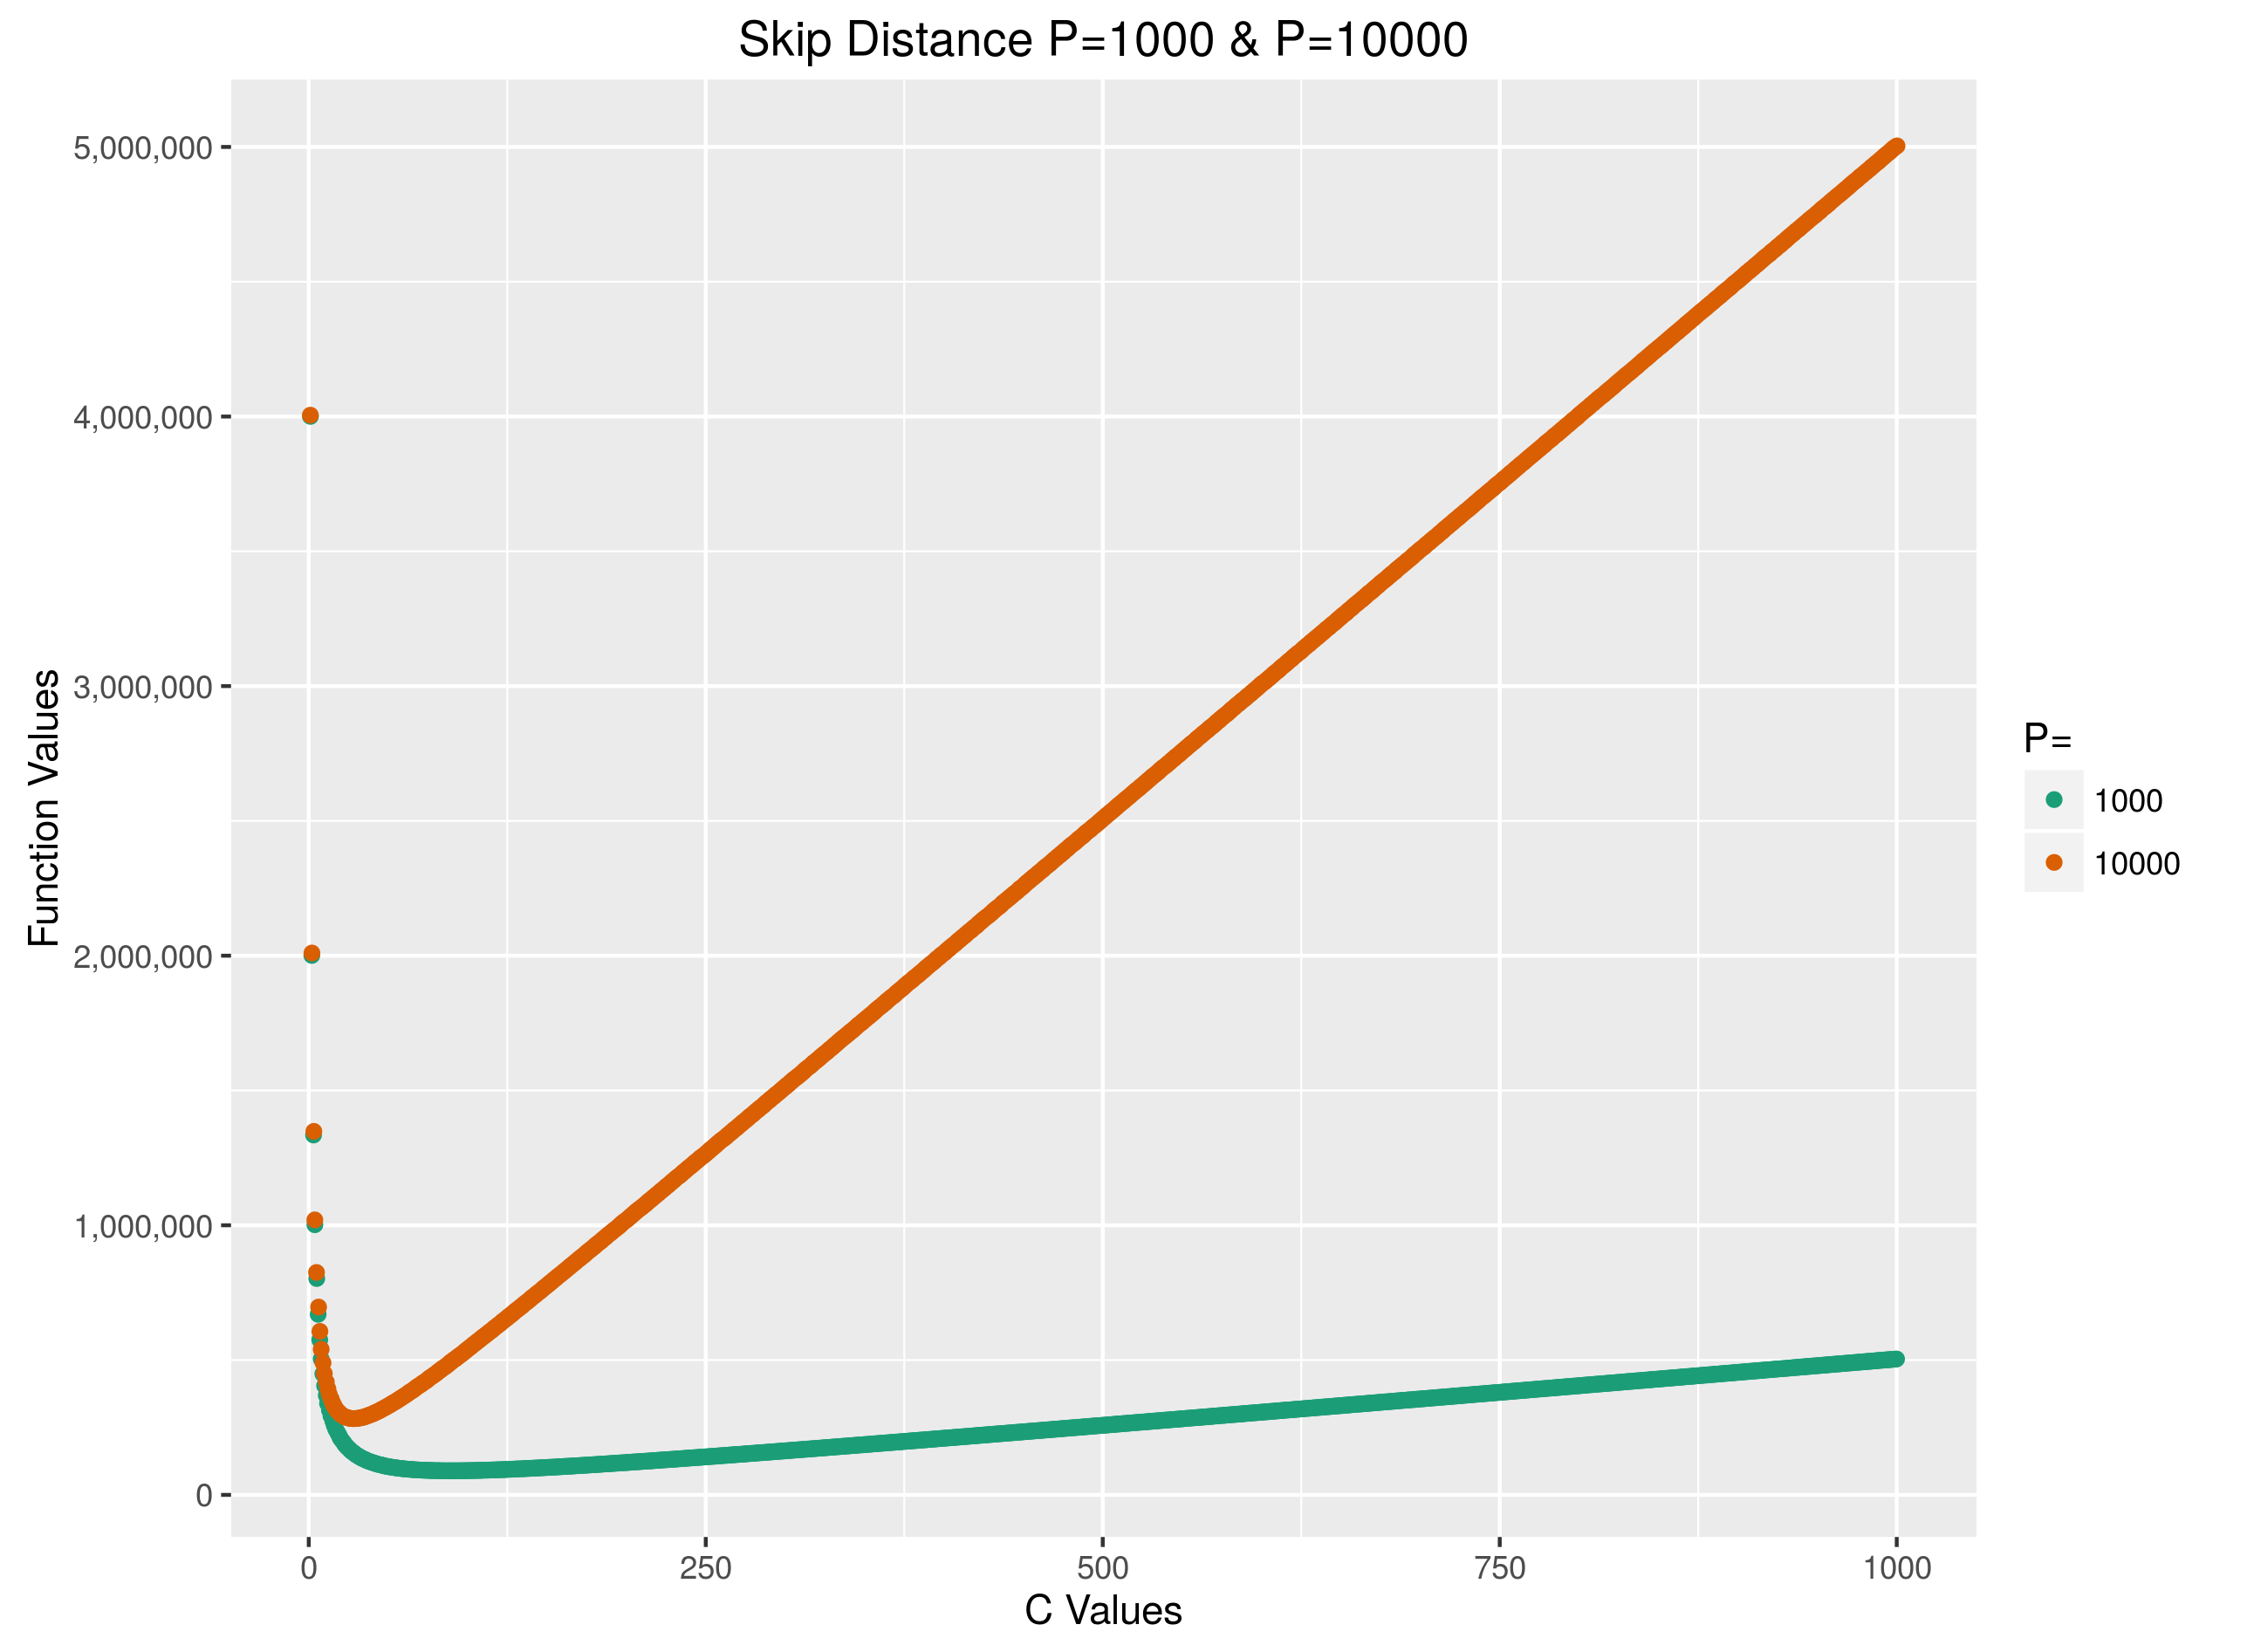
\includegraphics[width=\columnwidth]{code/skipDistanceBoth.png}
\caption{Skip Distance Optimal C Both P Plot}
\label{fig:skbp}
\end{figure}
\begin{figure}[h]
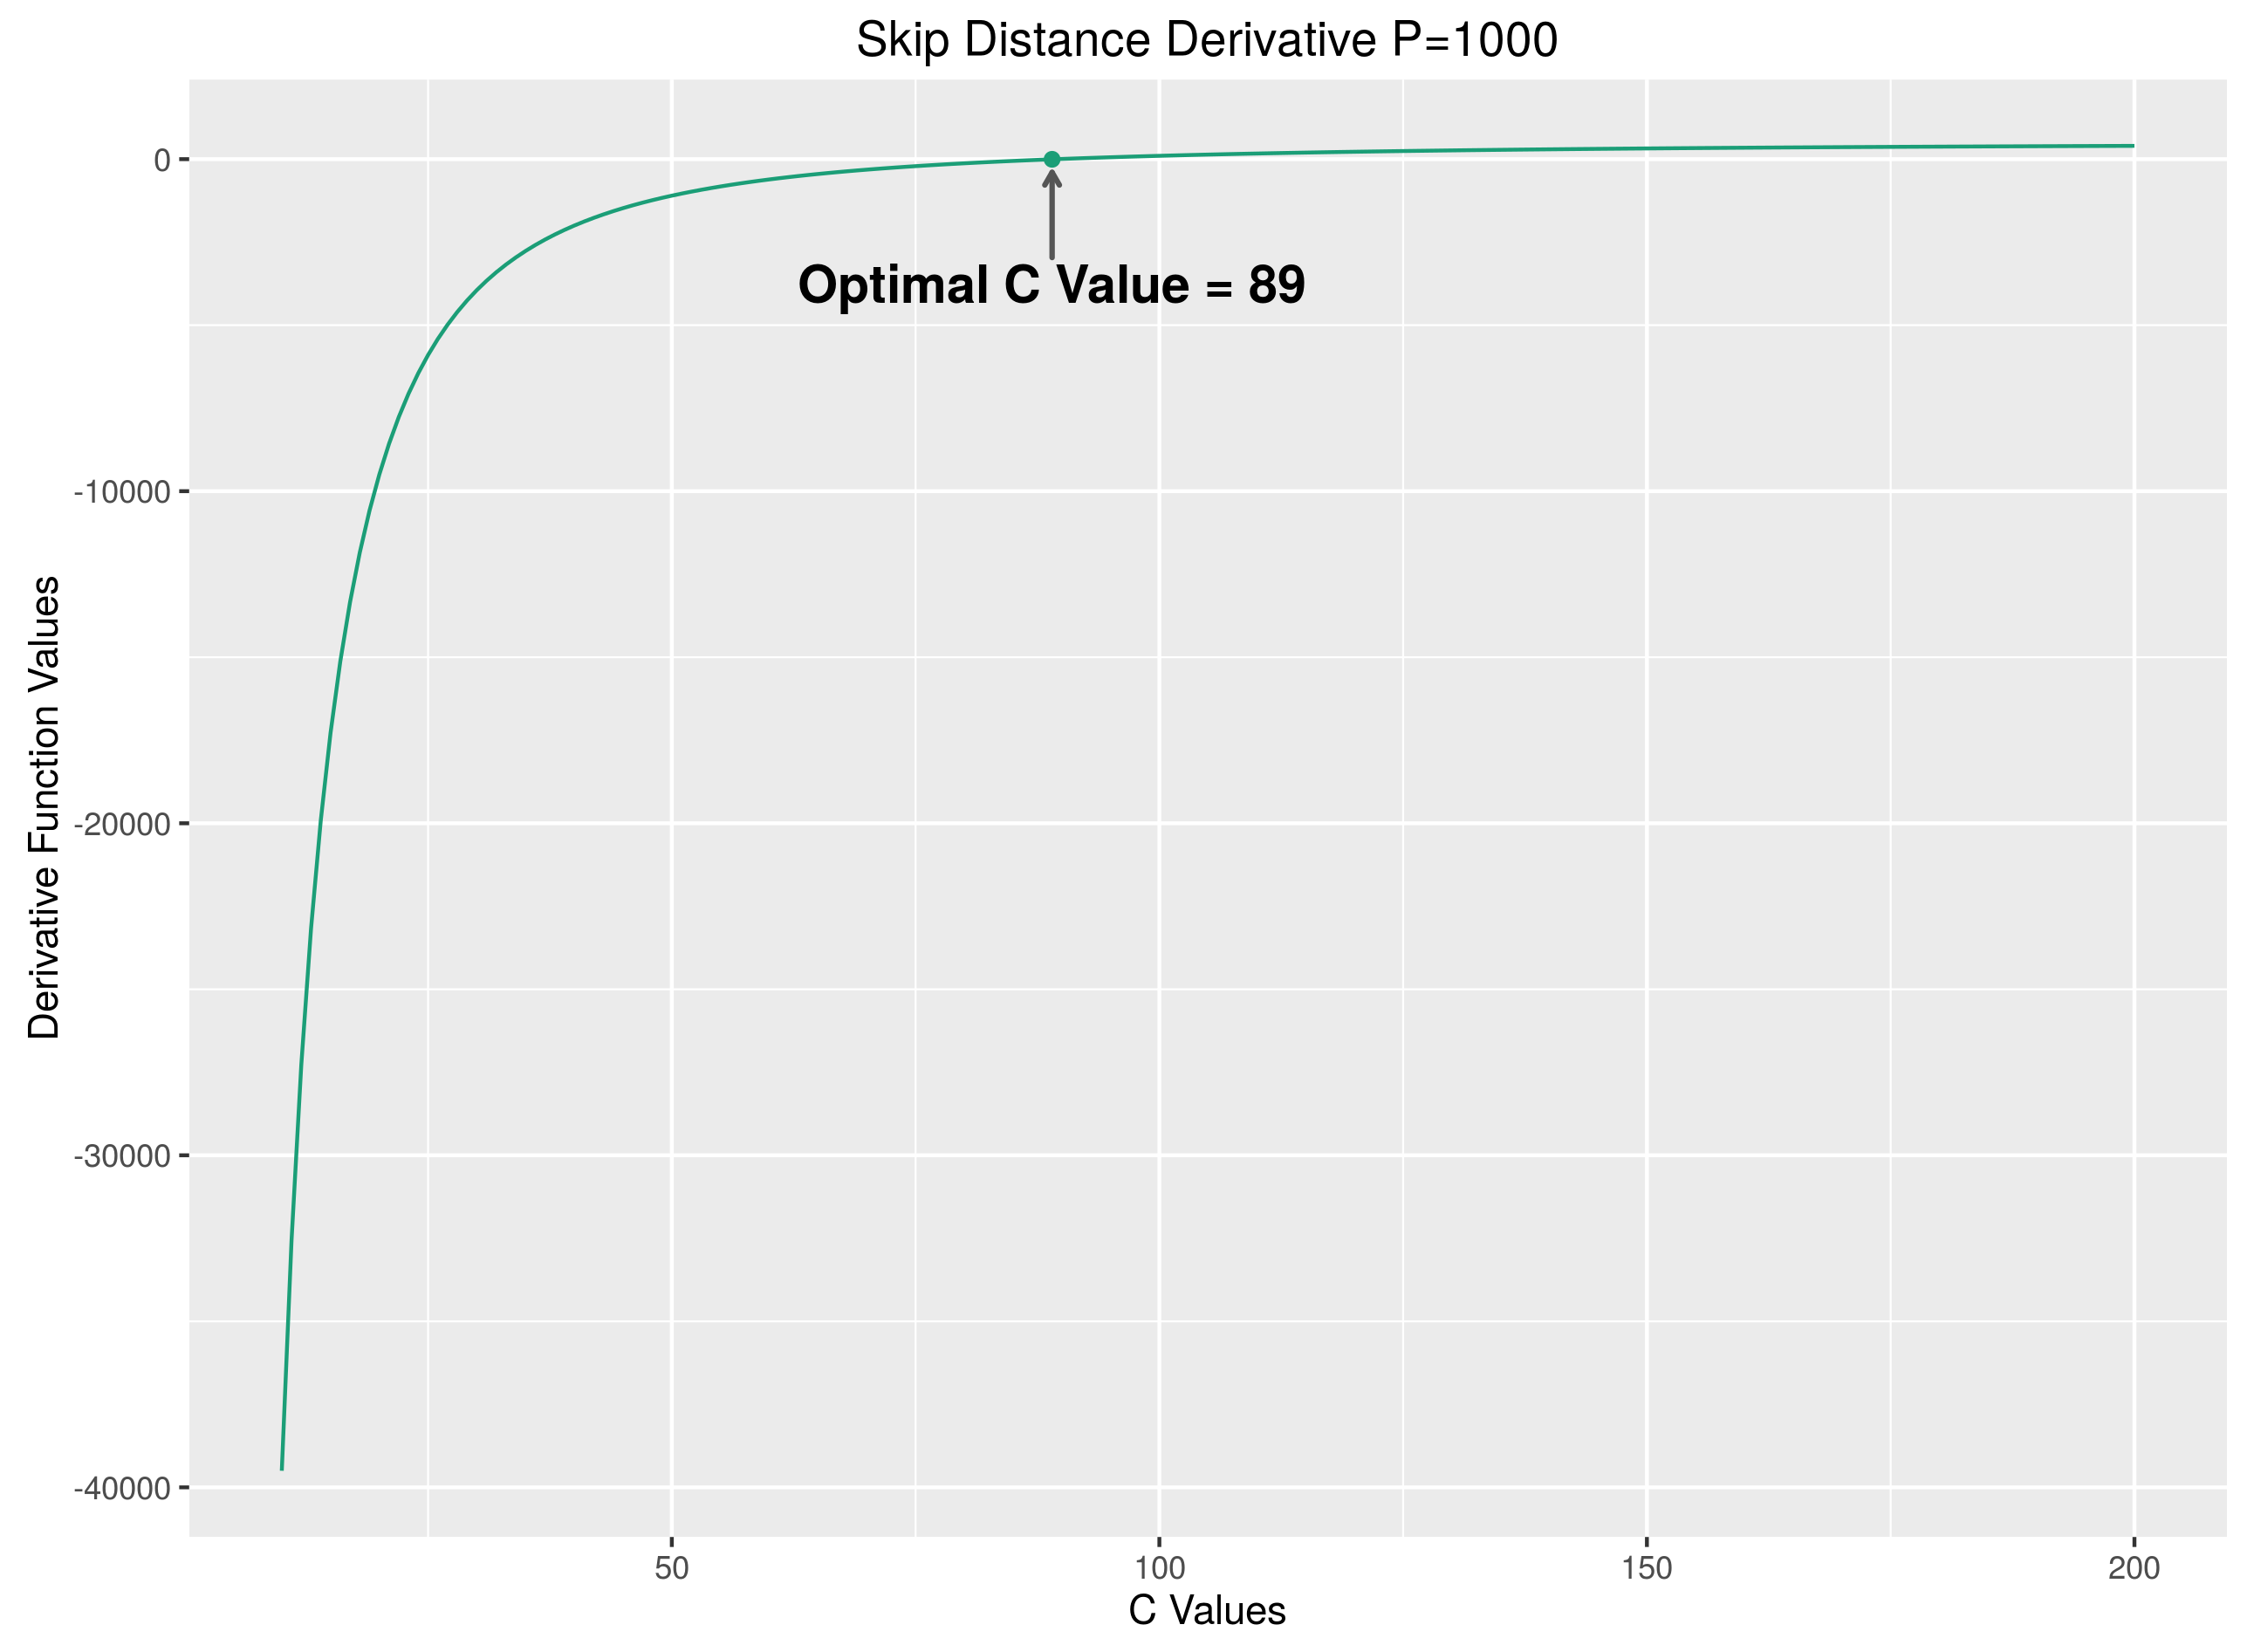
\includegraphics[width=\columnwidth]{code/skipDistanceD.png}
\caption{Skip Distance Derivative P=1000 Plot}
\label{fig:skdp}
\end{figure}
\begin{figure}[h]
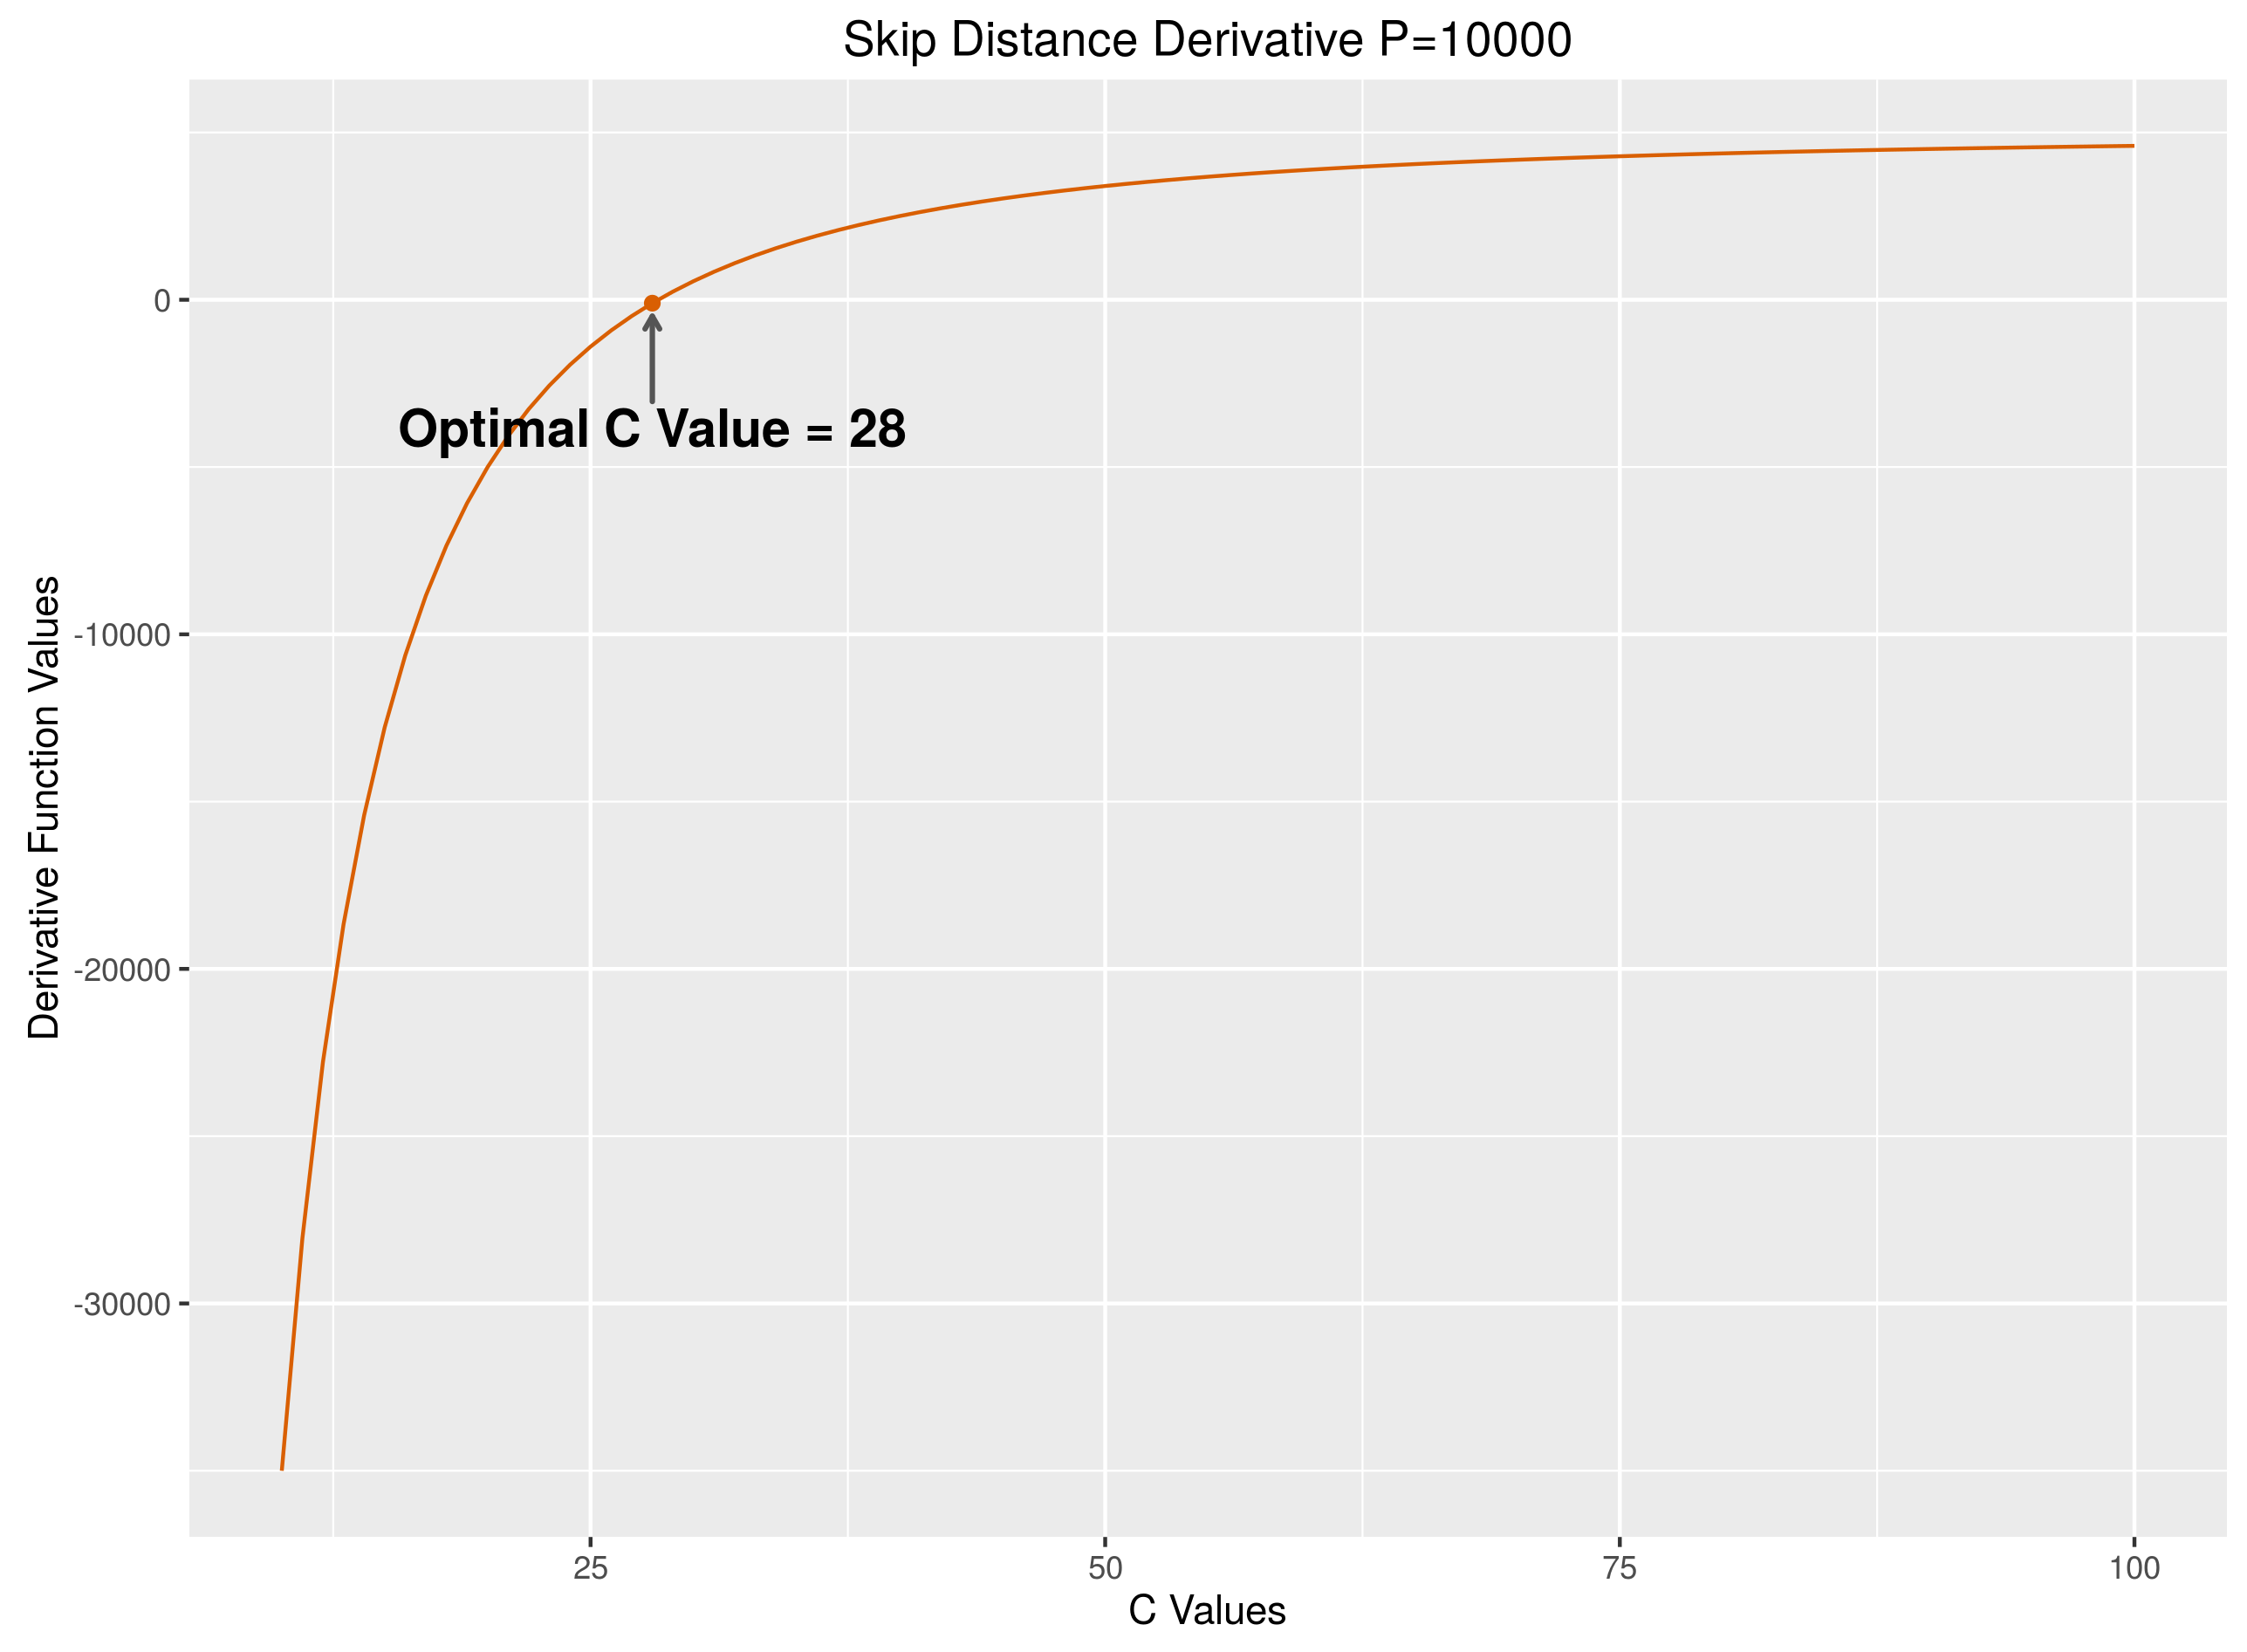
\includegraphics[width=\columnwidth]{code/skipDistanceD2.png}
\caption{Skip Distance Derivative P=10000 Plot}
\label{fig:skdp2}
\end{figure}
\newpage
\clearpage
\begin{code}
	\rcode{code/derivative.R}
	\captionof{listing}{First Derivative Of Skip Distance} \label{code:dsd}
\end{code}
\begin{code}
	\rcode{code/skip_distance.R}
	\captionof{listing}{Skip Distance Plots} \label{code:skip}
\end{code}
\newpage
\begin{code}
	\pycode{code/util.py}
	\captionof{listing}{Util File} \label{code:util}
\end{code}
\end{document}